\appendix
\clearpage
\section{Appendix}

\subsection{Proof of Lemma \ref{lemma:lora}} \label{sec:proof_lemma}

\begin{proof}
    Consider fine-tuning $B$ while freezing $A = Q$. The loss function in Eq. (\ref{eq:lr_loss}) becomes: 
    \begin{equation} \label{eq:lr_loss_fix_a}
        \mathcal{L} = \mathbb{E}_{(x_{t}, y_{t})}[\|y_{t} - (W_0 + BQ) x_{t} \|_2^2].
    \end{equation}
Then, the gradient of Eq. (\ref{eq:lr_loss_fix_a}) w.r.t. $B$ is:
\begin{equation} \label{eq:grad_b}
\begin{aligned}
    \frac{\partial \mathcal{L}}{\partial B} &=  \frac{\partial \mathbb{E}_{(x_{t}, y_{t})}[\|y_{t} - (W_0 + BQ) x_{t} \|_2^2]}{\partial B} \\
    &= \frac{\partial \mathbb{E}[\|W_tx_t - (W_0 + BQ) x_{t} \|_2^2]}{\partial B} \\
    &= \frac{\partial \mathbb{E}[\|(W_0 + \Delta_W)x_t - (W_0 + BQ) x_{t} \|_2^2]}{\partial B} \\
    &= \frac{\partial \mathbb{E}[\|(\Delta_W - BQ)x_t \|_2^2]}{\partial B} \\
    &= \mathbb{E}[2[(\Delta_W - BQ)x_t] (-x_t^T Q^T)] \\
    &= \mathbb{E}[2(BQ - \Delta_W) x_{t}x_t^T Q^T].
\end{aligned}
\end{equation}
To obtain the optimal $B^*$, we set Eq. (\ref{eq:grad_b}) to zero, which means:
\begin{equation}
\begin{aligned}
    \mathbb{E}[2(BQ - \Delta_W) x_{t}x_t^T Q^T] &= 0 \\
    2BQ\mathbb{E}[x_tx_t^T]Q^T - 2\Delta_W\mathbb{E}[x_tx_t^T]Q^T &= 0 \\
    2BQ\mathbb{E}[x_tx_t^T]Q^T - 2\Delta_W\mathbb{E}[x_tx_t^T]Q^T &= 0 \\
    BQ\mathbb{E}[x_tx_t^T]Q^T &= \Delta_W\mathbb{E}[x_tx_t^T]Q^T  \\
    B &= \Delta_W\mathbb{E}[x_tx_t^T]Q^T (Q\mathbb{E}[x_tx_t^T]Q^T)^{-1}.
\end{aligned}
\end{equation}
Therefore, we obtain $B^*= \Delta_W\mathbb{E}[x_tx_t^T]Q^T (Q\mathbb{E}[x_tx_t^T]Q^T)^{-1}$.

When fine-tuning $A$ with fixed $B = U$. The loss function in Eq. (\ref{eq:lr_loss}) becomes:
    \begin{equation} \label{eq:lr_loss_fix_b}
        \mathcal{L} = \mathbb{E}_{(x_{t}, y_{t})}[\|y_{t} - (W_0 + UA) x_{t} \|_2^2].
    \end{equation}
Then, the gradients of Eq. (\ref{eq:lr_loss_fix_a}) w.r.t. $A$ is:
\begin{equation} \label{eq:grad_a}
\begin{aligned}
    \frac{\partial \mathcal{L}}{\partial A} &=  \frac{\partial \mathbb{E}_{(x_{t}, y_{t})}[\|y_{t} - (W_0 + UA) x_{t} \|_2^2]}{\partial A} \\
    &= \frac{\partial \mathbb{E}[\|W_tx_t - (W_0 + UA) x_{t} \|_2^2]}{\partial A} \\
    &= \frac{\partial \mathbb{E}[\|(W_0 + \Delta_W)x_t - (W_0 + BQ) x_{t} \|_2^2]}{\partial A} \\
    &= \frac{\partial \mathbb{E}[\|(\Delta_W - UA)x_t \|_2^2]}{\partial A} \\
    &= \mathbb{E}[2U^T[(\Delta_W - UA)x_t]x_t^T] \\
\end{aligned}
\end{equation}
To obtain the optimal $A^*$, we set Eq. (\ref{eq:grad_a}) to zero, which means:
\begin{equation}
\begin{aligned}
    \mathbb{E}[2U^T[(\Delta_W - UA)x_t]x_t^T] &= 0 \\
    2U^T\Delta_W \mathbb{E}[x_tx_t^T] - 2U^TUA \mathbb{E}[x_tx_t^T] &= 0\\
    U^TUA \mathbb{E}[x_tx_t^T] &= U^T\Delta_W \mathbb{E}[x_tx_t^T] \\
    A &= U^{-1}\Delta_W.
\end{aligned}
\end{equation}
Thus, we obtain $A^*= U^{-1}\Delta_W$.
\end{proof}

\subsection{Proof of Theorem \ref{theorem1}} \label{sec:proof_theorem}
\begin{proof}
Let $W_i^{(t)}=W_0+B_i^{(t)}A_i^{(t)}$ be the model parameters maintained in the $i$-th client at the $t$-th step. Let $\mathcal{I}_E$ be the set of global synchronization steps, i.e., $\mathcal{I}_E=\{nE \mid n=1,2,\cdots\}$. If $t+1 \in \mathcal{I}_E$, which represents the time step for communication, then the one-step update of the proposed method for the $i$-th client can be described as follows:
\begin{equation*}
% \begin{array}{c}
\left(\begin{array}{c}
B_i^{(t)} \\
A_i^{(t)}
\end{array}\right) \underset{\text{update  of } B_i^{(t)} \text{and} A_i^{(t)}}{\longrightarrow}\left(\begin{array}{c}
B_i^{(t+1)} \\
A_i^{(t+1)}
\end{array}\right) \underset{\text { if } t+1 \in \mathcal{I}_E}{\longrightarrow}\left(\begin{array}{c}
B_i^{(t+1)} \\
\frac{1}{m}\sum_{j=1}^m A_j^{(t+1)}
\end{array}\right).
% \end{array}
\end{equation*}
For convenience, we denote the parameters in each sub-step above as follows:
\begin{equation*}
\begin{aligned}
% \begin{array}{c}
W_i^{(t)} &= W_0 + B_i^{(t)}A_i^{(t)}, \\
U_i^{(t)} &= W_0 + B_i^{(t+1)}A_i^{(t+1)}, \\
V_i^{(t)} &= W_0 + B_i^{(t+1)} \frac{1}{m} \sum_{j=1}^m A_j^{(t+1)}, \\
% \end{array}.
% \end{equation*}
% \begin{equation*}
W_i^{(t+1)} &= \begin{cases}U_i^{(t)} & \text { if } t+1 \notin \mathcal{I}_E, \\ V_i^{(t)} & \text { if } t+1 \in \mathcal{I}_E.\end{cases}
\end{aligned}
\end{equation*}
Here, the variable $U_i^{(t)}$ represents the immediate result of one sub-step update from the parameter of the previous sub-step $W_i^{(t)}$, and $V_i^{(t)}$ represents the parameter obtained after communication steps (if applicable).
Furthermore, we denote the learning rate for the $i$-th client at the $t$-th step as $\eta_{i,t}$, and the stochastic gradient at step $t$ as follows:
\begin{equation*}
% \begin{array}{c}
\begin{aligned}
\nabla_{B}\mathcal{L}_i(W_i^{(t)},\xi_{i,t}) &= \nabla_{W}\mathcal{L}_i(W_i^{(t)},\xi_{i,t}){A_i^{(t)}}^{\top}, \\
\nabla_{A}\mathcal{L}_i(W_i^{(t)},\xi_{i,t}) &= {B_i^{(t)}}^{\top}\nabla_{W}\mathcal{L}_i(W_i^{(t)},\xi_{i,t}), \\
\nabla_{B}\mathcal{L}_i(W_i^{(t)}) &= \mathbb{E}[\nabla_{B}\mathcal{L}_i(W_i^{(t)},\xi_{i,t})], \\
\nabla_{A}\mathcal{L}_i(W_i^{(t)}) &= \mathbb{E}[\nabla_{A}\mathcal{L}_i(W_i^{(t)},\xi_{i,t})], \\
% \nabla_{W}\mathcal{L}_i(W_i^{(t)}) &= \mathbb{E}[\nabla_{W}\mathcal{L}_i(W_i^{(t)},\xi_{i,t})],
% \end{array}
\end{aligned}
\end{equation*}
where $\xi_{i,t}$ is the data uniformly chosen from the local data set of client $i$ at step $t$.

Next, we apply the inequality from the smoothness Assumption \ref{assumption1} to each sub-step of the one-step update for client $i$.
Firstly, by the smoothness of $\mathcal{L}_i$, we have:
\begin{equation}\label{l-smooth1}
\mathcal{L}_i(U_i^{(t)}) \leq \mathcal{L}_i(W_i^{(t)})+\langle U_i^{(t)}-W_i^{(t)}, \nabla_{W}\mathcal{L}_i(W_i^{(t)})\rangle_F+\frac{L}{2}\left\|U_i^{(t)}-W_i^{(t)}\right\|^2_F.
\end{equation}
% where $\langle \cdot,\cdot \rangle$ denotes the Frobenius inner product.
Since
\begin{equation*}
\begin{aligned}
B_i^{(t+1)} &= B_i^{(t)} - \eta_{i,t}\nabla_{B}\mathcal{L}_i(W_i^{(t)},\xi_{i,t})\\
&= B_i^{(t)} - \eta_{i,t} \nabla_{W}\mathcal{L}_i(W_i^{(t)},\xi_{i,t}){A_i^{(t)}}^{\top},
\end{aligned}
\end{equation*}
and
\begin{align*}
A_i^{(t+1)} &= A_i^{(t)} - \eta_{i,t}\nabla_{A}\mathcal{L}_i(W_i^{(t)},\xi_{i,t})\\
&= A_i^{(t)} - \eta_{i,t}{B_i^{(t)}}^{\top}\nabla_{W}\mathcal{L}_i(W_i^{(t)},\xi_{i,t}),
\end{align*}
we have:
\begin{equation} \label{u_w_difference}
\begin{aligned}
& U_i^{(t)}-W_i^{(t)} \notag\\
= \ & B_i^{(t+1)}A_i^{(t+1)}-B_i^{(t)}A_i^{(t)}\notag\\
= \ & \left(B_i^{(t)} - \eta_{i,t}\nabla_{W}\mathcal{L}_i(W_i^{(t)},\xi_{i,t}){A_i^{(t)}}^{\top}\right)\left(A_i^{(t)} - \eta_{i,t}{B_i^{(t)}}^{\top}\nabla_{W}\mathcal{L}_i(W_i^{(t)},\xi_{i,t})\right) - B_i^{(t)}A_i^{(t)}\notag\\
= \ & \eta_{i,t}^2 \nabla_{W}\mathcal{L}_i(W_i^{(t)},\xi_{i,t}){A_i^{(t)}}^{\top}{B_i^{(t)}}^{\top}\nabla_{W}\mathcal{L}_i(W_i^{(t)},\xi_{i,t})- \eta_{i,t}\nabla_{W}\mathcal{L}_i(W_i^{(t)},\xi_{i,t}){A_i^{(t)}}^{\top}A_i^{(t)}\notag\\
& - \eta_{i,t}B_i^{(t)}{B_i^{(t)}}^{\top}\nabla_{W}\mathcal{L}_i(W_i^{(t)},\xi_{i,t}).
\end{aligned}
\end{equation}
Then, for the second term on the right side of Eq. (\ref{l-smooth1}), according to the law of total expectation, we have:
\begin{align*}
& \mathbb{E}\left[\left\langle U_i^{(t)}-W_i^{(t)}, \nabla_{W}\mathcal{L}_i(W_i^{(t)})\right\rangle_F\right]\\
= \ & \eta_{i,t}^2 \mathbb{E}\left[\left\langle \nabla_{W}\mathcal{L}_i(W_i^{(t)},\xi_{i,t}){A_i^{(t)}}^{\top}{B_i^{(t)}}^{\top}\nabla_{W}\mathcal{L}_i(W_i^{(t)},\xi_{i,t}),\nabla_{W}\mathcal{L}_i(W_i^{(t)})\right\rangle_F\right]\\
& - \eta_{i,t}\mathbb{E}\left[\left\langle \nabla_{W}\mathcal{L}_i(W_i^{(t)},\xi_{i,t}){A_i^{(t)}}^{\top}A_i^{(t)},\nabla_{W}\mathcal{L}_i(W_i^{(t)})\right\rangle_F\right]\\
& - \eta_{i,t}\mathbb{E}\left[\left\langle B_i^{(t)}{B_i^{(t)}}^{\top}\nabla_{W}\mathcal{L}_i(W_i^{(t)},\xi_{i,t}),\nabla_{W}\mathcal{L}_i(W_i^{(t)})\right\rangle_F\right]\\
= \ & \eta_{i,t}^2 \left\langle \nabla_{W}\mathcal{L}_i(W_i^{(t)}){A_i^{(t)}}^{\top}{B_i^{(t)}}^{\top}\nabla_{W}\mathcal{L}_i(W_i^{(t)}),\nabla_{W}\mathcal{L}_i(W_i^{(t)})\right\rangle_F\\
& - \eta_{i,t}\left\langle \nabla_{W}\mathcal{L}_i(W_i^{(t)}){A_i^{(t)}}^{\top}A_i^{(t)},\nabla_{W}\mathcal{L}_i(W_i^{(t)})\right\rangle_F\\
& - \eta_{i,t}\left\langle B_i^{(t)}{B_i^{(t)}}^{\top}\nabla_{W}\mathcal{L}_i(W_i^{(t)}),\nabla_{W}\mathcal{L}_i(W_i^{(t)})\right\rangle_F.
\end{align*}
Since
\begin{align*}
& \left\langle \nabla_{W}\mathcal{L}_i(W_i^{(t)}){A_i^{(t)}}^{\top}{B_i^{(t)}}^{\top}\nabla_{W}\mathcal{L}_i(W_i^{(t)}),\nabla_{W}\mathcal{L}_i(W_i^{(t)})\right\rangle_F\\
\leq \ & \left\| \nabla_{W}\mathcal{L}_i(W_i^{(t)}){A_i^{(t)}}^{\top}{B_i^{(t)}}^{\top}\nabla_{W}\mathcal{L}_i(W_i^{(t)})\right\|\left\|\nabla_{W}\mathcal{L}_i(W_i^{(t)})\right\|_F\\
\leq \ & \left\|{A_i^{(t)}}\right\|\left\|{B_i^{(t)}}\right\|_F\left\|\nabla_{W}\mathcal{L}_i(W_i^{(t)})\right\|_F^3\\
\leq \ & C_A C_B G^3,
\end{align*}
and if we 
%denote $A_i^{(t)}=(a_{i,1}^{(t)},\ldots,a_{i,d}^{(t)})$ and 
assume there exists $c_A > 0$ such that $\forall t$:
\begin{equation*}
\Big\langle {A_i^{(t)}}^{\top}A_i^{(t)}, \nabla_{W}\mathcal{L}_i(W_i^{(t)})^{\top}\nabla_{W}\mathcal{L}_i(W_i^{(t)})\Big\rangle_F
\geq c_A \left\|\nabla_{W}\mathcal{L}_i(W_i^{(t)})\right\|_F^2,
\end{equation*}
then we have:
\begin{align*}
\left\langle \nabla_{W}\mathcal{L}_i(W_i^{(t)}){A_i^{(t)}}^{\top}A_i^{(t)},\nabla_{W}\mathcal{L}_i(W_i^{(t)})\right\rangle_F 
= \ &  \text{Tr}\Big[\Big(\nabla_{W}\mathcal{L}_i(W_i^{(t)}){A_i^{(t)}}^{\top}A_i^{(t)}\Big)^{\top}\nabla_{W}\mathcal{L}_i(W_i^{(t)})\Big]\\
= \ &  \text{Tr}\Big[{A_i^{(t)}}^{\top}A_i^{(t)}\nabla_{W}\mathcal{L}_i(W_i^{(t)})^{\top}\nabla_{W}\mathcal{L}_i(W_i^{(t)})\Big]\\
= \ & \Big\langle {A_i^{(t)}}^{\top}A_i^{(t)}, \nabla_{W}\mathcal{L}_i(W_i^{(t)})^{\top}\nabla_{W}\mathcal{L}_i(W_i^{(t)})\Big\rangle_F\\
\geq \ & c_A \left\|\nabla_{W}\mathcal{L}_i(W_i^{(t)})\right\|_F^2.
\end{align*}
And similarly if we assume there exists $c_B > 0$ such that $\forall t$:
\begin{equation*}
\Big\langle {B_i^{(t)}}^{\top}B_i^{(t)}, \nabla_{W}\mathcal{L}_i(W_i^{(t)})^{\top}\nabla_{W}\mathcal{L}_i(W_i^{(t)})\Big\rangle_F
\geq c_B \left\|\nabla_{W}\mathcal{L}_i(W_i^{(t)})\right\|_F^2,
\end{equation*}
then we have:
\begin{align}\label{inner_product_1}
\left\langle B_i^{(t)}{B_i^{(t)}}^{\top}\nabla_{W}\mathcal{L}_i(W_i^{(t)}),\nabla_{W}\mathcal{L}_i(W_i^{(t)})\right\rangle_F \notag
= \ & \text{Tr}\Big[\Big(B_i^{(t)}{B_i^{(t)}}^{\top}\nabla_{W}\mathcal{L}_i(W_i^{(t)})\Big)^{\top}\nabla_{W}\mathcal{L}_i(W_i^{(t)})\Big]\notag\\
= \ & \text{Tr}\Big[\nabla_{W}\mathcal{L}_i(W_i^{(t)})^{\top}B_i^{(t)}{B_i^{(t)}}^{\top}\nabla_{W}\mathcal{L}_i(W_i^{(t)})\Big] \notag\\
= \ & \text{Tr}\Big[\nabla_{W}\mathcal{L}_i(W_i^{(t)})\nabla_{W}\mathcal{L}_i(W_i^{(t)})^{\top}B_i^{(t)}{B_i^{(t)}}^{\top}\Big] \notag\\
= \ & \left\langle \nabla_{W}\mathcal{L}_i(W_i^{(t)})\nabla_{W}\mathcal{L}_i(W_i^{(t)})^{\top}, B_i^{(t)}{B_i^{(t)}}^{\top}\right\rangle_F \notag\\
\geq \ & c_B \Big\|\nabla_{W}\mathcal{L}_i(W_i^{(t)})\Big\|_F^2,
\end{align}
where we use the cyclic property of the trace for the third equality above.
We further get:
\begin{align}\label{inner_product_2}
& \mathbb{E}\left[\left\langle U_i^{(t)}-W_i^{(t)}, \nabla_{W}\mathcal{L}_i(W_i^{(t)})\right\rangle_F\right]\notag\\
\leq \ & \eta_{i,t}^2 C_A C_B G^3 - \eta_{i,t} c_A^2 \left\|\nabla_{W}\mathcal{L}_i(W_i^{(t)})\right\|_F^2 - \eta_{i,t} c_B^2 \left\|\nabla_{W}\mathcal{L}_i(W_i^{(t)})\right\|_F^2.
\end{align}
Similarly, we know:
\begin{align}\label{diff-square-norm}
\mathbb{E}[\|U_i^{(t)}-W_i^{(t)}\|_F^2] \notag
= \ & \mathbb{E}[\|\eta_{i,t}^2 \nabla_{W}\mathcal{L}_i(W_i^{(t)},\xi_{i,t}){A_i^{(t)}}^{\top}{B_i^{(t)}}^{\top}\nabla_{W}\mathcal{L}_i(W_i^{(t)},\xi_{i,t}) \notag \\
& - \eta_{i,t}\nabla_{W}\mathcal{L}_i(W_i^{(t)},\xi_{i,t}){A_i^{(t)}}^{\top}A_i^{(t)} - \eta_{i,t}B_i^{(t)}{B_i^{(t)}}^{\top}\nabla_{W}\mathcal{L}_i(W_i^{(t)},\xi_{i,t})\|_F^2] \notag \\
\leq \ & 3\eta_{i,t}^4 C_A^2 C_B^2G^4+3\eta_{i,t}^2 C_A^2 G^2 + 3\eta_{i,t}^2 C_B^2 G^2.
\end{align}
Plugging Eq. (\ref{inner_product_1}), Eq. (\ref{inner_product_2}), and Eq. (\ref{diff-square-norm}) into Eq. (\ref{l-smooth1}), we have:
\begin{align}\label{main-ineq-1}
\mathcal{L}_i\left(U_i^{(t)}\right) \notag
\leq \ &\mathcal{L}_i\left(W_i^{(t)}\right)+\eta_{i,t}^2 C_A C_B G^3 - \eta_{i,t} c_A \left\|\nabla_{W}\mathcal{L}_i(W_i^{(t)})\right\|_F^2 - \eta_{i,t} c_B \left\|\nabla_{W}\mathcal{L}_i(W_i^{(t)})\right\|_F^2 \notag\\
&+\frac{3}{2}\eta_{i,t}^4 C_A^2 C_B^2G^4L+\frac{3}{2}\eta_{i,t}^2 C_A^2 G^2L + \frac{3}{2}\eta_{i,t}^2 C_B^2 G^2L.
\end{align}
Secondly, by the smoothness of $\mathcal{L}_i$, we have:
\begin{equation}\label{l-smooth2}
\mathcal{L}_i\left(V_i^{(t)}\right) \leq \mathcal{L}_i\left((U_i^{(t)}\right)+\left\langle V_i^{(t)}-U_i^{(t)}, \nabla_{W}\mathcal{L}_i(U_i^{(t)})\right\rangle_F+\frac{L}{2}\left\|V_i^{(t)}-U_i^{(t)}\right\|^2_F.
\end{equation}
Since
\begin{equation*}
\begin{aligned}
V_i^{(t)} - U_i^{(t)}
& = B_i^{(t+1)}A_i^{(t+1)} - \frac{1}{m}B_i^{(t+1)}\sum_{j=1}^m A_j^{(t+1)}\\
& = B_i^{(t+1)}\frac{1}{m}\sum_{j=1}^m\Big(A_i^{(t+1)} - A_j^{(t+1)}\Big),
\end{aligned}
\end{equation*}
and 
\begin{align*}
A_j^{(t+1)} 
& = A_j^{(t-E+1)} - \sum_{t_0=t-E+1}^t \eta_{j,t_0} \nabla_A \mathcal{L}_j(W_j^{(t_0)};\xi_{j,t_0})\\
& = A_j^{(t-E+1)} - \sum_{t_0=t-E+1}^t \eta_{j,t_0}{B_j^{(t_0)}}^{\top} \nabla_W \mathcal{L}_j(W_j^{(t_0)};\xi_{j,t_0}),
\end{align*}
we know:
\begin{align*}
V_i^{(t)} - U_i^{(t)} = B_i^{(t+1)} \Big(-\frac{1}{m}\sum_{j=1}^m \sum_{t_0=t-E+1}^t \eta_{j,t_0}{B_j^{(t_0)}}^{\top}\big(\nabla \mathcal{L}_i(W_i^{(t_0)};\xi_{i,t_0})-\nabla \mathcal{L}_j(W_j^{(t_0)};\xi_{j,t_0})\big)\Big).
\end{align*}
Therefore,
\begin{align}\label{diff-square-norm-2}
& \mathbb{E}\Big[\Big\|V_i^{(t)}-U_i^{(t)}\Big\|_F^2\Big] \notag\\
= \ & \mathbb{E}\Big[\Big\|B_i^{(t+1)}\Big\|_F^2 \Big\|-\frac{1}{m}\sum_{j=1}^m \sum_{t_0=t-E+1}^t \eta_{j,t_0}{B_j^{(t_0)}}^{\top}\big(\nabla \mathcal{L}_i(W_i^{(t_0)};\xi_{i,t_0})-\nabla \mathcal{L}_j(W_j^{(t_0)};\xi_{j,t_0})\big)\Big\|_F^2\Big]\notag\\
\leq \ & C_B^2 \frac{E}{m}\sum_{j=1}^m \sum_{t_0=t-E+1}^t \eta_{j,t_0}^2 \mathbb{E}\Big[\Big\|{B_j^{(t_0)}}^{\top}\big(\nabla \mathcal{L}_i(W_i^{(t_0)};\xi_{i,t_0})-\nabla \mathcal{L}_j(W_j^{(t_0)};\xi_{j,t_0})\big)\Big\|_F^2\Big]\notag\\
\leq \ & \frac{C_B^4 E}{m}\sum_{j=1}^m \sum_{t_0=t-E+1}^t \eta_{j,t_0}^2 \mathbb{E}\Big[\Big\|\nabla \mathcal{L}_i(W_i^{(t_0)};\xi_{i,t_0})-\nabla \mathcal{L}_j(W_j^{(t_0)};\xi_{j,t_0})\Big\|_F^2\Big]\notag\\
\leq \ & \frac{4C_B^4 E G^2}{m}\sum_{j=1}^m \sum_{t_0=t-E+1}^t \eta_{j,t_0}^2,
\end{align}
where we use Assumption \ref{assumption2} to derive that:
\begin{align*}
& \mathbb{E}\Big[\Big\|\nabla \mathcal{L}_i(W_i^{(t_0)};\xi_{i,t_0})-\nabla \mathcal{L}_j(W_j^{(t_0)};\xi_{j,t_0})\Big\|_F^2\Big] \\
\leq \ & 2\mathbb{E}\Big[\Big\|\nabla \mathcal{L}_i(W_i^{(t_0)};\xi_{i,t_0})\Big\|_F^2\Big]+ 2\mathbb{E}\Big[\Big\|\nabla \mathcal{L}_i(W_j^{(t_0)};\xi_{j,t_0})\Big\|_F^2\Big]\\
\leq \ & 4G^2.
\end{align*}
Furthermore, 
\begin{align}\label{inner_product_3}
\left\langle V_i^{(t)}-U_i^{(t)}, \nabla_W L_i(U_i^{(t)})\right\rangle \notag
\leq \ & \frac{1}{2\eta_{i,t}}\Big\|V_i^{(t)}-U_i^{(t)}\Big\|_F^2 + \frac{1}{2}\eta_{i,t}\Big\|\nabla_W \mathcal{L}_i(U_i^{(t)})\Big\|_F^2 \notag\\
\leq \ & \frac{2C_B^4 E G^2}{\eta_{i,t}m}\sum_{j=1}^m \sum_{t_0=t-E+1}^t \eta_{j,t_0}^2 + \frac{1}{2}\eta_{i,t}G^2.
\end{align}
Plugging Eq. (\ref{diff-square-norm-2}) and Eq. (\ref{inner_product_3}) into Eq. (\ref{l-smooth2}), we have (choose constant learning rate $\eta_{i,t}=\eta$):
\begin{align}\label{main-ineq-2}
\mathcal{L}_i\left(V_i^{(t)}\right) \leq \mathcal{L}_i\left(U_i^{(t)}\right)+\big(2C_B^2E^2G^2+\frac{1}{2}G^2\big)\eta+2\eta^2C_B^4 E^2 G^2L.
\end{align}
Combining Eq. (\ref{main-ineq-1}) and Eq. (\ref{main-ineq-2}), we have (choose constant learning rate $\eta_{i,t}=\eta$):
\begin{align*}
\mathcal{L}_i\left(W_i^{(t+1)}\right) 
\leq \ & \mathcal{L}_i\left((W_i^{(t)}\right)
+ (2C_B^2E^2G^2+\frac{1}{2}G^2)\eta + \frac{3}{2}\eta^4 C_A^2 C_B^2G^4L\\
&+(C_A C_B G^2+\frac{3}{2}C_A^2L G^2+\frac{3}{2}C_B^2L G^2+2C_B^4 E^2 L G^2)\eta^2\\
&- \eta (c_A+c_B) \left\|\nabla_{W}\mathcal{L}_i(W_i^{(t)})\right\|^2,
\end{align*}
which is equivalent to:
\begin{align*}
\eta (c_A+c_B) \left\|\nabla_{W}\mathcal{L}_i(W_i^{(t)})\right\|_F^2 
\leq \ & \mathcal{L}_i\left((W_i^{(t)}\right)-\mathcal{L}_i\left(W_i^{(t+1)}\right)\\
&+ (2C_B^2E^2G^2+\frac{1}{2}G^2)\eta + \frac{3}{2}\eta^4 C_A^2 C_B^2G^4L\\
&+(C_A C_B G^2+\frac{3}{2}C_A^2L G^2+\frac{3}{2}C_B^2L G^2+2C_B^4 E^2 L G^2)\eta^2.
\end{align*}
Choosing $M$ which satisfies $(2C_B^2E^2G^2+\frac{1}{2}G^2)\eta + \frac{3}{2}\eta^4 C_A^2 C_B^2G^4L+(C_A C_B G^2+\frac{3}{2}C_A^2L G^2+\frac{3}{2}C_B^2L G^2+2C_B^4 E^2 L G^2)\eta^2 \leq M\eta^2$, we get:
\begin{align}\label{main-ineq-3}
\left\|\nabla_{W}\mathcal{L}_i(W_i^{(t)})\right\|_F^2 
\leq \ & \frac{\mathcal{L}_i\left((W_i^{(t)}\right)-\mathcal{L}_i\left(W_i^{(t+1)}\right)}{\eta(c_A+c_B)}+\frac{M\eta}{c_A+c_B}.
\end{align}
Now, by repeatedly applying Eq. (\ref{main-ineq-3}) for different values of $t$ and summing up the results, we get:
\begin{align}\label{main-ineq-4}
\sum_{t=1}^T\left\|\nabla_{W}\mathcal{L}_i(W_i^{(t)})\right\|_F^2 
\leq & \frac{\mathcal{L}_i\left((W_i^{(1)}\right)-\mathcal{L}_i\left(W_i^{*}\right)}{\eta(c_A^2+c_B^2)}+\eta \frac{M}{c_A+c_B}T.
\end{align}
Dividing both side of Eq. (\ref{main-ineq-4}) by $T$, we get:
\begin{align}\label{main-ineq-5}
\frac{1}{T}\sum_{t=1}^T\left\|\nabla_{W}\mathcal{L}_i(W_i^{(t)})\right\|_F^2 
\leq & \frac{\mathcal{L}_i\left((W_i^{(1)}\right)-\mathcal{L}_i\left(W_i^{*}\right)}{\eta(c_A+c_B)T}+\eta \frac{M}{c_A+c_B}.
\end{align}
Let us assume that $\mathcal{L}_i(W_i^{(1)})-\mathcal{L}_i(W_i^{*}) \leq D, \forall i$, and we set $\eta = \sqrt{\frac{D}{MT}}$. Then, we have:
\begin{align}\label{main-ineq-6}
\frac{1}{T}\sum_{t=1}^T\left\|\nabla_{W}\mathcal{L}_i(W_i^{(t)})\right\|_F^2 
\leq & \frac{2}{c_A+c_B}\sqrt{\frac{DM}{T}}.
\end{align}
Thus, we can obtain:
\begin{align}\label{main-ineq-7}
\frac{1}{mT}\sum_{i=1}^m \sum_{t=1}^T\left\|\nabla_{W}\mathcal{L}_i(W_i^{(t)})\right\|_F^2 
\leq & \frac{2}{c_A+c_B}\sqrt{\frac{DM}{T}}.
\end{align}
\end{proof}

\subsection{Further Explanations about Aggregation Errors.} \label{app_sec:aggregation_error}

In this section, we provide more explanation about what aggregation errors are and why people do not achieve the ``ideal'' model update.

When introducing LoRA into FL, the update for the $i$-the client is given by $\Delta_{W_i} =  B_i A_i$. The ``ideal'' model update for server aggregation should be:
\begin{equation} \label{eq:ideal}
\Delta_{W}^* = \frac{1}{m}\sum_{i=1}^{m}\Delta_{W_i} = \frac{1}{m}\sum_{i=1}^{m}B_i A_i = \frac{1}{m}(B_1A_1 + B_2A_2 + \cdots + B_mA_m). 
\end{equation}
However, in practical LoRA training, the matrices $A_i$ and $B_i$, not the original $W_i$, are trainable. Thus, we cannot directly average the $\Delta_{W_i}$; instead, we can only separately average $A_i$ and $B_i$, and then combine them to obtain the update: 
\begin{equation}
\begin{aligned}
\Delta_{W} = & (\frac{1}{m}\sum_{i=1}^{m}B_i) (\frac{1}{m}\sum_{i=1}^{m}A_i) \\ 
= & \frac{1}{m}(B_1 + B_2 + \cdots + B_m)\frac{1}{m}(A_1 + A_2 + \cdots + A_m) \\
= & \frac{1}{m^2} (B_1A_1 + B_1A_2 + \cdots + B_1A_m + B_2A_1 \\
& + B_2A_2 + \cdots + B_2A_m + \cdots + B_mA_1 + B_mA_2 + \cdots + B_mA_m),
\end{aligned}
\end{equation}
which differs from the ``ideal'' model update in Eq. (\ref{eq:ideal}). This difference introduces aggregation errors.

Regarding why the ``ideal'' model update is not achieved, it is because the matrices $A_i$ and $B_i$ are trainable, not the original $W_i$. While it is possible to first combine $A_i$ and $B_i$ to obtain $\Delta_{W_i}$ and then average them to achieve the ``ideal'' update, we cannot decompose $W$ back into $A$ and $B$ for further federated training. This limitation prevents people from performing the ``ideal'' model update.


\subsection{Hyperparameters}

Tables \ref{tab:lr_lora} and \ref{tab:lr_rslora} show the learning rates used for LoRA-based methods and rsLoRA-based methods, respectively. For the VeRA-based methods, we first tried using the SGD optimizer \citep{ruder2016overview} with a search learning rate from $\eta \in \{5\text{E-}3, 1\text{E-}2, 2\text{E-}2, 5\text{E-}2, 1\text{E-}1\}$ as adopted in LoRA-based methods, but we found the performance to be significantly worse than that of LoRA-based methods. For example, the best performance among the three VeRA-based methods (i.e., VeRA, FFA-VeRA, and FedSA-VeRA) is 53.73\% on the MNLI-m task, which is significantly worse than that of the LoRA-based methods (90.20\%). Thus, we chose the AdamW optimizer \citep{Loshchilov2017DecoupledWD} and introduced separate learning rates for the classification head and the adapted layers as used in VeRA \citep{kopiczko2024vera}. The learning rates used for VeRA-based methods are shown in Table \ref{tab:lr_vera}.


\begin{table}[h]
\caption{The learning rates used for LoRA-based methods on the GLUE benchmark.}
\label{tab:lr_lora}
\begin{center}
% \resizebox{\linewidth}{!}{
\begin{tabular}{lcccccc}
\toprule 
 Method & MNLI-m & MNLI-mm & SST2 & QNLI & QQP & RTE \\
\midrule
LoRA & 1E-2 & 1E-2 & 2E-2 & 1E-2 & 1E-2 & 1E-2 \\
FFA-LoRA & 5E-2 & 5E-2 & 5E-2 & 2E-2 & 5E-2 & 2E-2 \\
\pengxin{FedDPA-LoRA} & \pengxin{1E-2} & \pengxin{1E-2} & \pengxin{1E-2} & \pengxin{5E-2} & \pengxin{5E-2} & \pengxin{1E-2} \\
FedSA-LoRA & 2E-2 & 2E-2 & 1E-2  & 5E-3 & 2E-2 & 1E-2 \\
\bottomrule
\end{tabular}
% }
\end{center}
\end{table}


\begin{table}[h]
\caption{The learning rates used for rsLoRA-based methods on the GLUE benchmark.}
\label{tab:lr_rslora}
\begin{center}
% \resizebox{\linewidth}{!}{
\begin{tabular}{lcccccc}
\toprule 
 Method & MNLI-m & MNLI-mm & SST2 & QNLI & QQP & RTE \\
\midrule
rsLoRA & 5E-3 & 5E-3 & 1E-2 & 2E-3 & 5E-3 & 2E-3 \\
FFA-rsLoRA & 2E-2 & 2E-2 & 2E-2 & 1E-2 & 2E-2 & 1E-2 \\
\pengxin{FedDPA-reLoRA} & \pengxin{5E-3} & \pengxin{5E-3} & \pengxin{1E-2} & \pengxin{1E-3} & \pengxin{5E-3} & \pengxin{1E-2} \\
FedSA-rsLoRA & 5E-3 & 5E-3 & 5E-3 & 1E-3 & 2E-3 & 2E-3 \\
\bottomrule
\end{tabular}
% }
\end{center}
\end{table}


\begin{table}[h]
\caption{The learning rates used for VeRA-based methods on the GLUE benchmark.}
\label{tab:lr_vera}
\begin{center}
% \resizebox{\linewidth}{!}{
\begin{tabular}{lccccccc}
\toprule 
 Method & Position & MNLI-m & MNLI-mm & SST2 & QNLI & QQP & RTE \\
\midrule
\multirow{2}{*}{VeRA} & VeRA & 1E-2 & 1E-2 & 2E-2 & 2E-3 & 2E-3 & 1E-2 \\
& Head & 6E-3 & 6E-3  & 2E-3 & 3E-4 & 3E-4 & 2E-4 \\
\midrule
\multirow{2}{*}{FFA-VeRA} & VeRA & 2E-2 & 2E-2 & 1E-2 & 1E-2 & 1E-2 & 1E-2 \\
& Head & 2E-3 & 2E-3 & 6E-3 & 2E-4 & 6E-3  & 2E-4 \\
\midrule 
\multirow{2}{*}{FedDPA-VeRA} & \pengxin{VeRA} & \pengxin{1E-2} & \pengxin{1E-2} & \pengxin{1E-2} & \pengxin{2E-3} & \pengxin{2E-2} & \pengxin{1E-2} \\
& \pengxin{Head} & \pengxin{6E-3} & \pengxin{6E-3} & \pengxin{6E-3} & \pengxin{3E-4} & \pengxin{2E-3} & \pengxin{2E-4} \\
\midrule
\multirow{2}{*}{FedSA-VeRA} & VeRA & 2E-3 & 2E-3 & 1E-2 & 1E-2 & 2E-3 & 1E-2 \\
& Head & 3E-5 & 3E-5 & 3E-4 & 3E-4 & 3E-4 & 1E-4 \\
\bottomrule
\end{tabular}
% }
\end{center}
\end{table}

\subsection{Examples of Generated Answer for GSM8K Datasets}

The results of the GSM8K dataset are shown in Table \ref{tab:result_nlg}, demonstrating that the proposed FedSA-LoRA outperforms other methods in complex natural language generation tasks. From the given example, it can be seen that both LoRA and FFA-LoRA have reasoning errors, but FedSA-LoRA can reason accurately, demonstrating the superiority of the proposed method.

\begin{table}[h]
\caption{Performance of different methods on the GSM8K dataset and example answers generated by each method.}
\label{tab:result_nlg}
\begin{center}
% \resizebox{\linewidth}{!}{
\begin{tabular}{l | p{3.6cm} | p{3.7cm} | p{3.6cm}}
\toprule 
  & \multicolumn{1}{c}{LoRA} & \multicolumn{1}{c}{FFA-LoRA} & \multicolumn{1}{c}{FedSA-LoRA} \\
\midrule
Accuracy & \multicolumn{1}{c}{46.24} & \multicolumn{1}{c}{46.32} & \multicolumn{1}{c}{\textbf{46.63}} \\ 
\midrule
Question: & \multicolumn{3}{p{11.5cm}}{In a student council election, candidate A got 20\% of the votes while candidate B got 50\% more than candidate A's votes. The rest of the votes was given to candidate C. If there were 100 voters, how many votes did candidate C get?} \\
\midrule
Output: & Candidate A got 20\% of the votes. That is 20\% of 100 = 20\% $\times$ 100 = 20 $\times$ 100 = 2000 votes. Candidate B got 50\% more than candidate A. That is 50\% of 2000 = 50\% $\times$ 2000 = 50 $\times$ 2000 = 10000 votes. The rest of the votes was given to candidate C. So there are 10000 + 2000 = 12000 votes in total. Candidate C got 10000 votes. The answer is 10000.  [\ding{56}] & 
Candidate A got 20\% of 100 = 100 $\times$ 20\% = 100 $\times$ 20/100 = 20. Candidate B got 20\% more than candidate A's votes, which is 20\% + 20\% = 40\%. 40\% of 100 = 100 $\times$ 40\% = 100 $\times$ 40/100 = 40. So the two candidates together got 20 + 40 = 60. The rest of the votes were given to candidate C. So candidate C got 100 - 60 = 40. The answer is 40. [\ding{56}] &
Candidate A got 20\% of the votes or 20\% $*$ 100 = 20 votes. Then candidate B got 50\% more than candidate A's 20 votes so 50\% of 20 is 20 $*$ 50\% = 10. Then candidate B got 20 + 10 = 30 votes. So candidate C got 100 - 20 - 30 = 50 votes. The answer is 50. [\ding{52}] \\
% \midrule
% Question: & \multicolumn{3}{p{11.5cm}}{A merchant wants to make a choice of purchase between 2 purchase plans: jewelry worth \$5,000 or electronic gadgets worth \$8,000. His financial advisor speculates that the jewelry market will go up 2.5\% while the electronic gadgets market will rise 1.2\% within the same month. If the merchant is looking to maximize profit at the end of this month by making a choice, how much profit would this be?} \\
% \midrule
% Output: & The jewerly would rise by 2.5\% = 5000 * 2.5\% = \$125. The electronic gadgets would rise by 1.2\% = 8000 $*$ 1.2\% = \$96. So the choice between the two options would be the electronic gadgets. It would rise by \$96 while the jewerly would rise by \$125. The answer is \$96. [\ding{56}] &
% The merchant must choose which purchase plan gives the largest profit. The profit is the difference between the purchase price and the sale price. If he buys jewelry, the profit would be \$5000 - 5000 $\times$ 2.5\% = \$5000 - 125 = \$4875. If he buys electronic gadgets, the profit would be \$8000 - 8000 $\times$ 1.2\% = \$8000 - 96 = \$7904. Since 7904 $>$ 4875, he should buy electronic gadgets. The answer is \$7904. [\ding{56}] & 
% He can buy 5,000 dollars worth of jewelry or 8,000 dollars worth of electronics. If he buys the 5,000 dollars of jewelry, his profit will be 5,000 $*$ 0.025 = 125. If he buys the 8,000 dollars worth of electronics, his profit will be 8,000 $*$ 0.012 = 96. The answer is 125. [\ding{52}] \\
\bottomrule
\end{tabular}
% }
\end{center}
\end{table}

\clearpage

\subsection{Learned Matrices Comparison}

% \subsubsection{Learned LoRA Query Matrices Comparison}

% In this section, we present the mean of pairwise client relationships for the learned LoRA query matrices in Figure \ref{fig:motivating_example_query_mean}. These results demonstrate a similar phenomenon to the learned value matrices shown in Figure \ref{fig:motivating_example_value_mean}. Specifically, the learned $A$ matrices are more similar than the $B$ matrices, and with increased data heterogeneity, the similarity of $B$ matrices between different clients decreases. These results indicate that the $A$ matrices are responsible for learning general knowledge, while the $B$ matrices focus on modeling client-specific knowledge.


% \begin{figure*}[h]
%   \centering
%     \subfigure[IID]{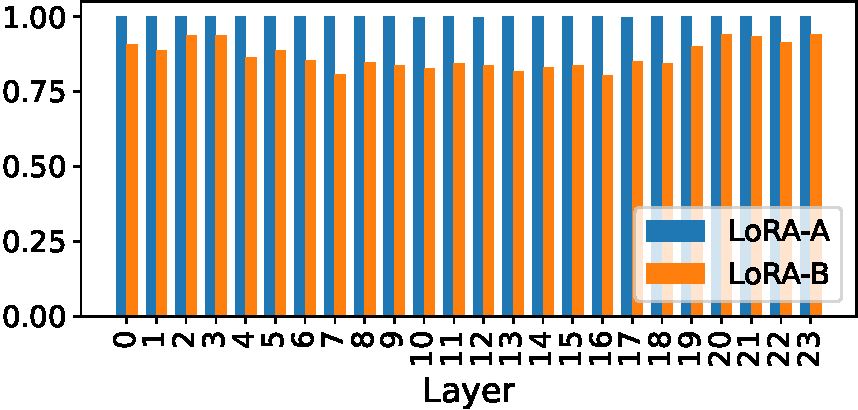
\includegraphics[width=0.32\linewidth]{rte_mean_query_iid.pdf}}
%     \subfigure[moderate non-IID]{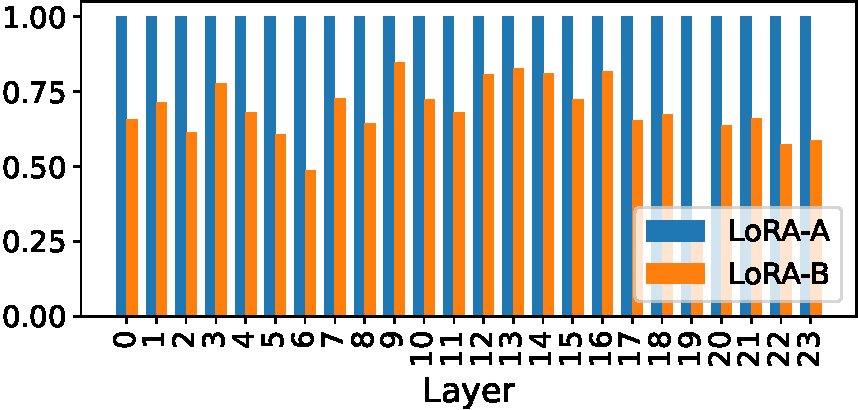
\includegraphics[width=0.32\linewidth]{rte_mean_query_lda_1.pdf}}
%     \subfigure[server non-IID]{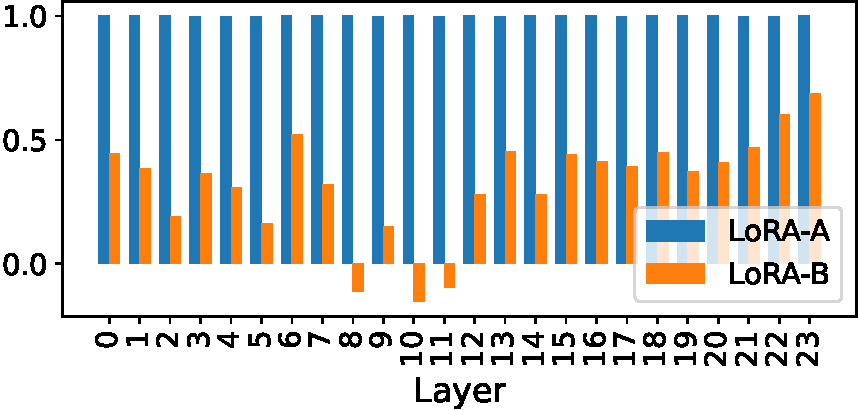
\includegraphics[width=0.32\linewidth]{rte_mean_query_lda_0.5.pdf}}
%   \caption{Mean of pairwise cosine similarity of the learned query $A$ and $B$ matrices across layers of a RoBERTa model locally fine-tuned with LoRA on the RTE task, with different levels of data heterogeneity.}
% \label{fig:motivating_example_query_mean}
% \end{figure*}

% \begin{figure*}[h]
%   \centering
%     \subfigure[Client 1 \& 2]{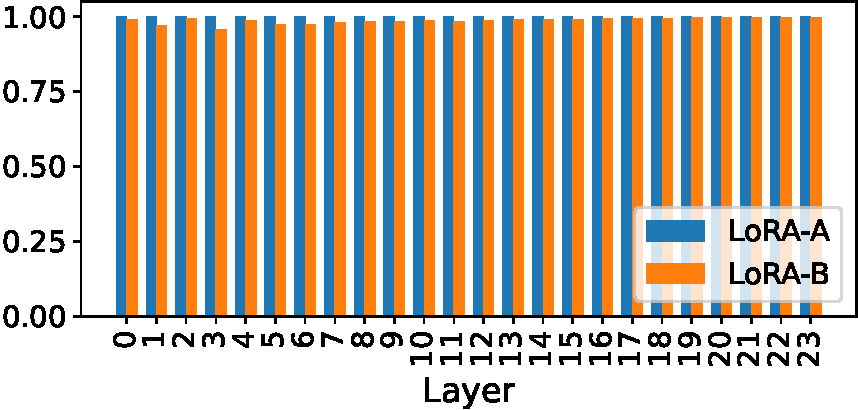
\includegraphics[width=0.32\linewidth]{rte_c1_c2_value_iid.pdf}}
%     \subfigure[Client 1 \& 3]{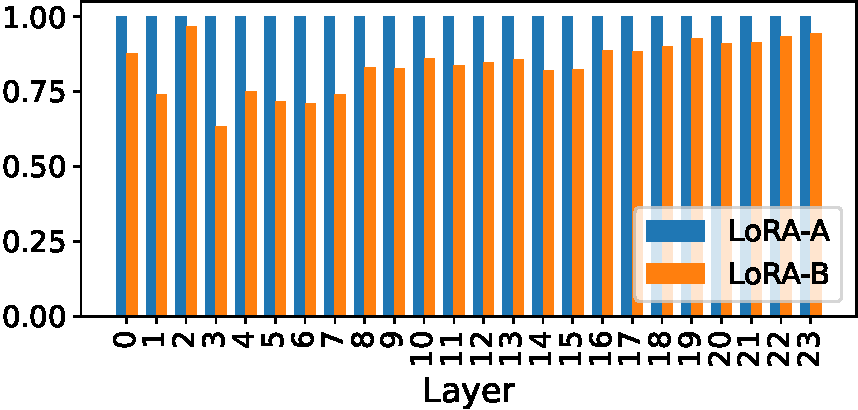
\includegraphics[width=0.32\linewidth]{rte_c1_c3_value_iid.pdf}}
%     \subfigure[Client 2 \& 3]{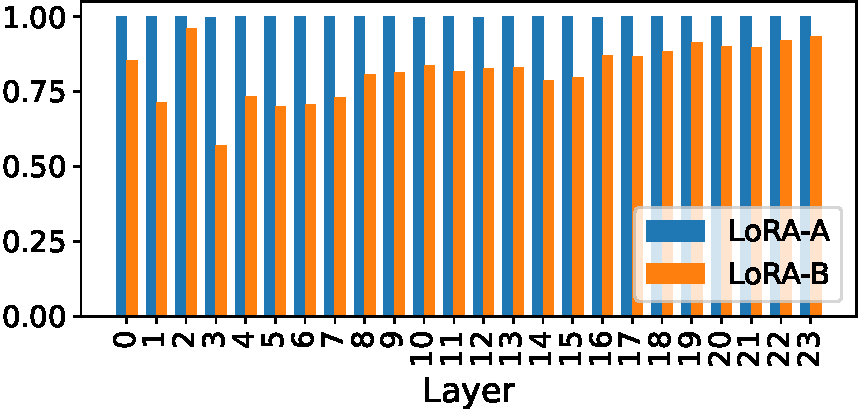
\includegraphics[width=0.32\linewidth]{rte_c2_c3_value_iid.pdf}}
%     \subfigure[Client 1 \& 2]{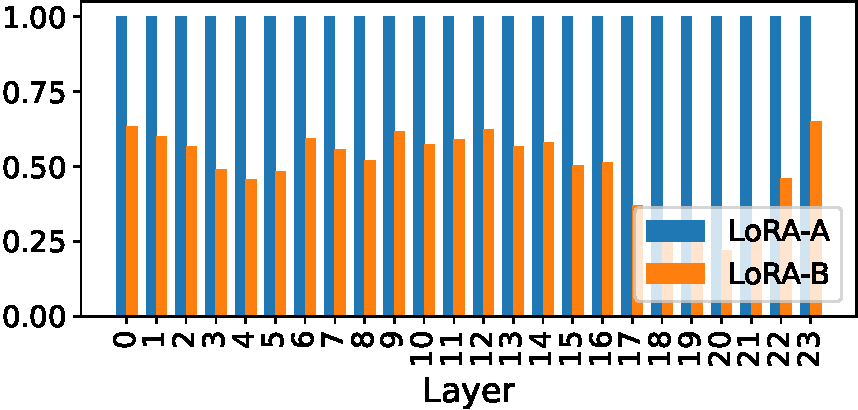
\includegraphics[width=0.32\linewidth]{rte_c1_c2_value_lda_1.pdf}}
%     \subfigure[Client 1 \& 3]{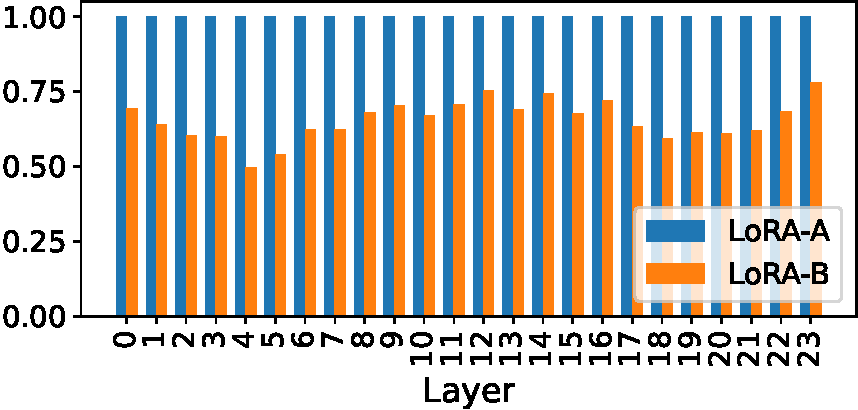
\includegraphics[width=0.32\linewidth]{rte_c1_c3_value_lda_1.pdf}}
%     \subfigure[Client 2 \& 3]{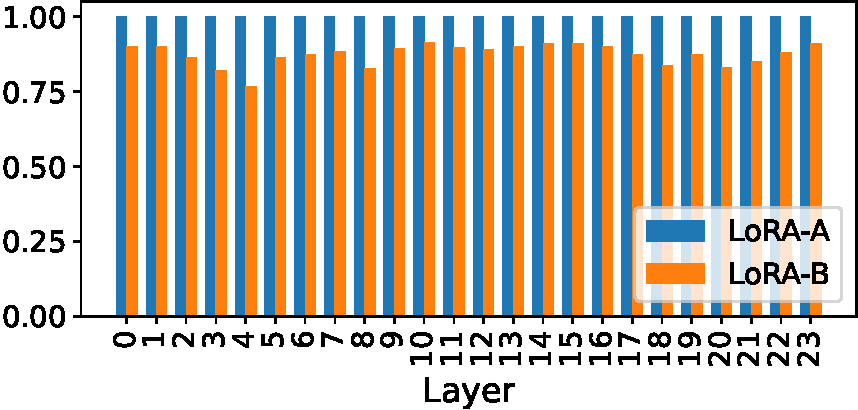
\includegraphics[width=0.32\linewidth]{rte_c2_c3_value_lda_1.pdf}}
%     \subfigure[Client 1 \& 2]{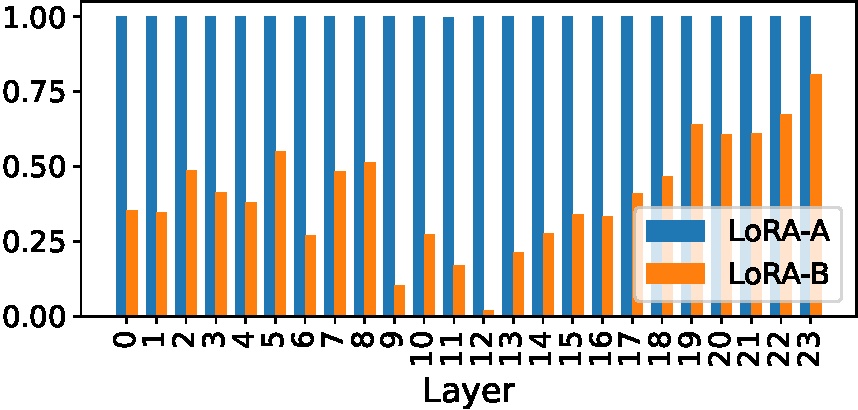
\includegraphics[width=0.32\linewidth]{rte_c1_c2_value_lda_0.5.pdf}}
%     \subfigure[Client 1 \& 3]{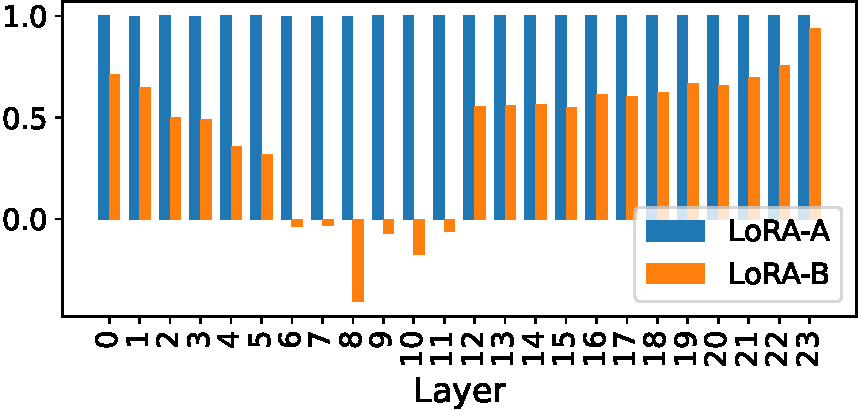
\includegraphics[width=0.32\linewidth]{rte_c1_c3_value_lda_0.5.pdf}}
%     \subfigure[Client 2 \& 3]{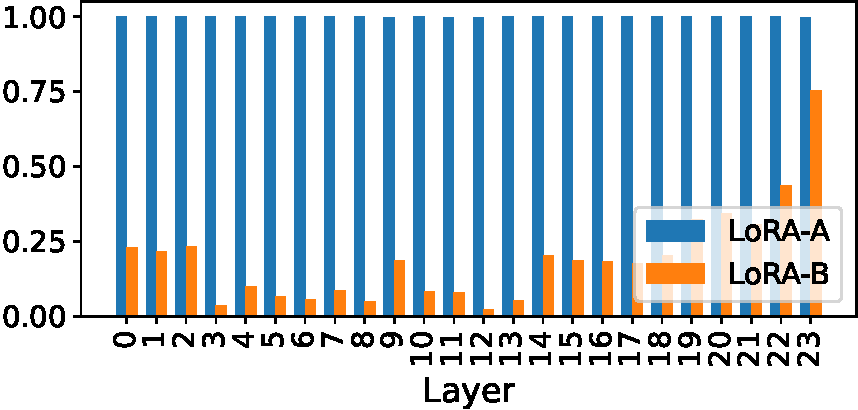
\includegraphics[width=0.32\linewidth]{rte_c2_c3_value_lda_0.5.pdf}}
%   \caption{Cosine similarity of learned value matrices $A$ \& $B$ across layers between different clients of a RoBERTa model locally fine-tuned with LoRA on the RTE task with different levels of data heterogeneity. (a)-(c): IID; (d)-(f): moderate non-IID; (g)-(i): severe non-IID.}
%   \label{fig:motivating_example_value}
% \end{figure*}

% \begin{figure*}[h]
%   \centering
%     \subfigure[Client 1 \& 2]{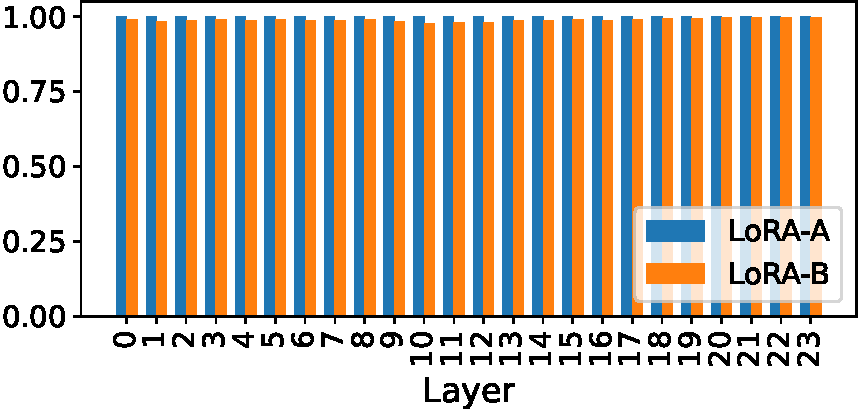
\includegraphics[width=0.32\linewidth]{rte_c1_c2_query_iid.pdf}}
%     \subfigure[Client 1 \& 3]{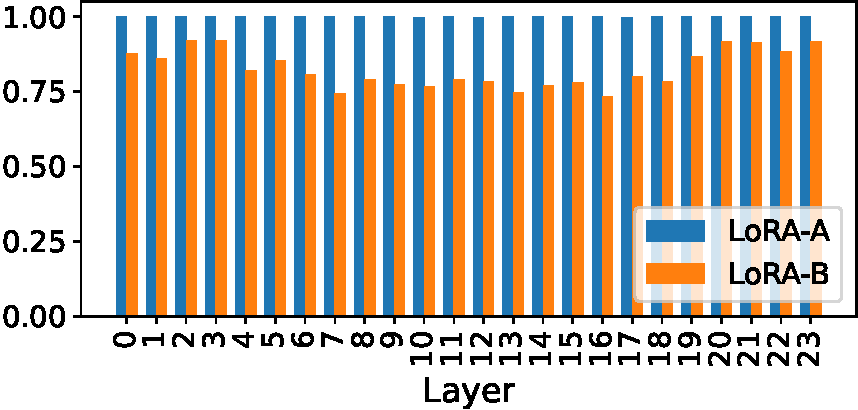
\includegraphics[width=0.32\linewidth]{rte_c1_c3_query_iid.pdf}}
%     \subfigure[Client 2 \& 3]{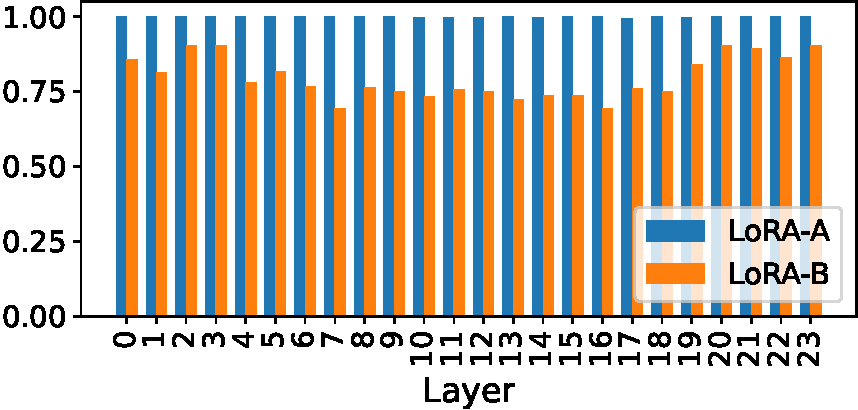
\includegraphics[width=0.32\linewidth]{rte_c2_c3_query_iid.pdf}}
%     \subfigure[Client 1 \& 2]{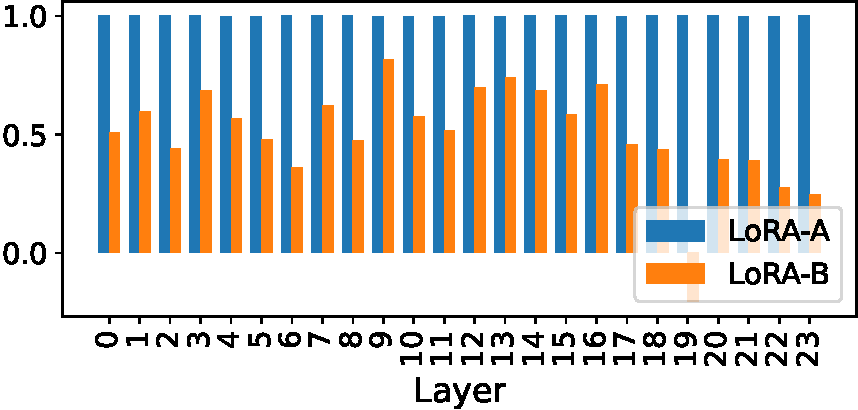
\includegraphics[width=0.32\linewidth]{rte_c1_c2_query_lda_1.pdf}}
%     \subfigure[Client 1 \& 3]{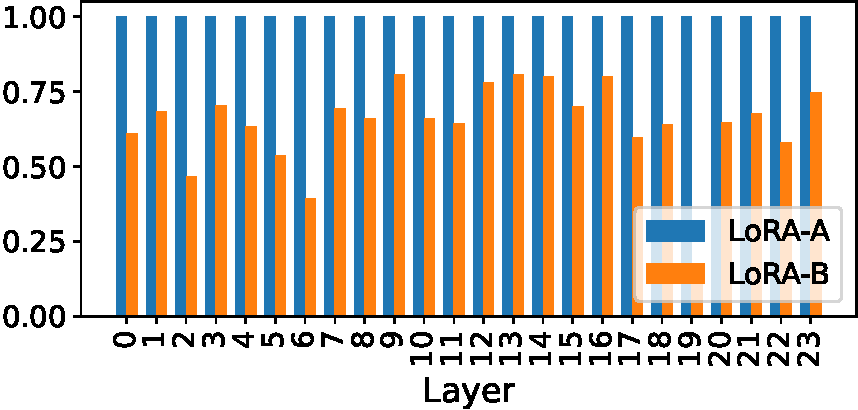
\includegraphics[width=0.32\linewidth]{rte_c1_c3_query_lda_1.pdf}}
%     \subfigure[Client 2 \& 3]{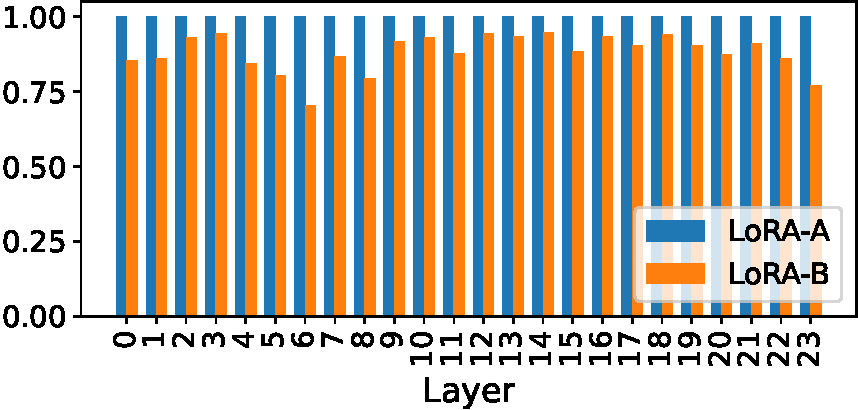
\includegraphics[width=0.32\linewidth]{rte_c2_c3_query_lda_1.pdf}}
%     \subfigure[Client 1 \& 2]{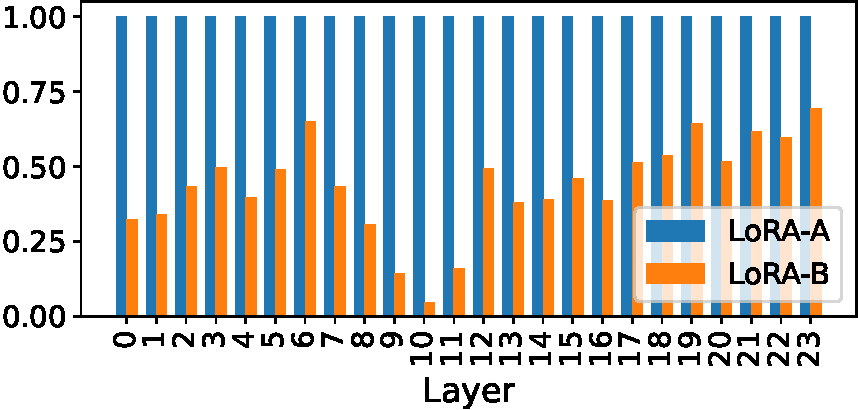
\includegraphics[width=0.32\linewidth]{rte_c1_c2_query_lda_0.5.pdf}}
%     \subfigure[Client 1 \& 3]{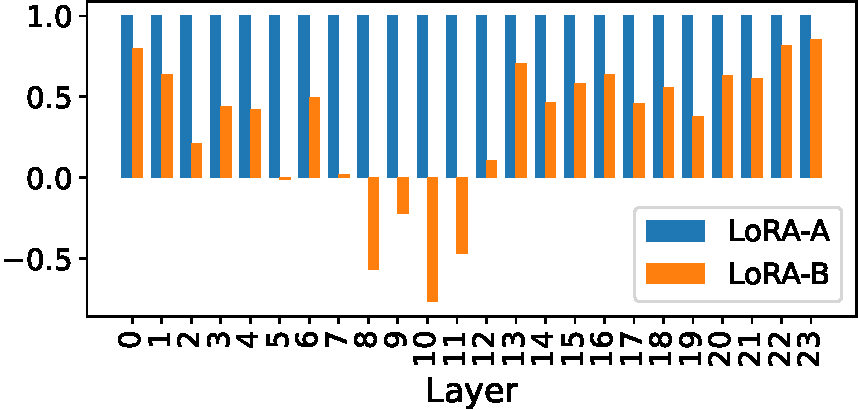
\includegraphics[width=0.32\linewidth]{rte_c1_c3_query_lda_0.5.pdf}}
%     \subfigure[Client 2 \& 3]{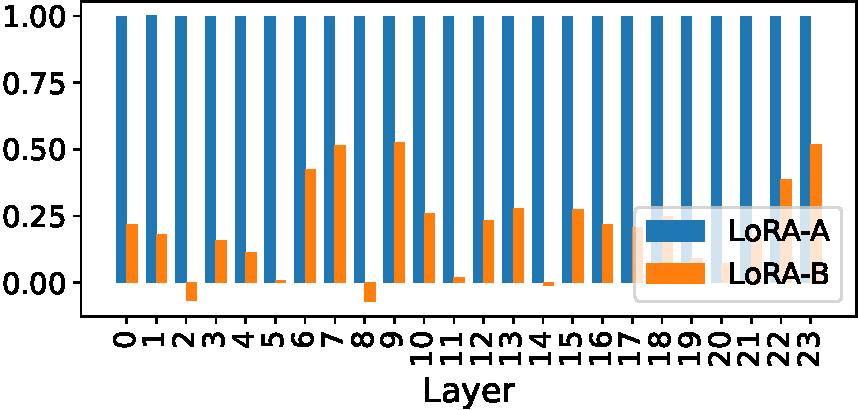
\includegraphics[width=0.32\linewidth]{rte_c2_c3_query_lda_0.5.pdf}}
%   \caption{Cosine similarity of learned query matrices $A$ \& $B$ across layers between different clients of a RoBERTa model locally fine-tuned with LoRA on the RTE task with different levels of data heterogeneity. (a)-(c): IID; (d)-(f): moderate non-IID; (g)-(i): severe non-IID.}
%   \label{fig:motivating_example_query}
% \end{figure*}


\subsubsection{Learned and Initialized LoRA Matrices Comparison}

Since the learned LoRA $A$ matrices are similar across different clients in Figure \ref{fig:motivating_example_mean}, \pengxin{we separately plotted the relationships of $A$ from Figure \ref{fig:motivating_example_mean} in Figure \ref{fig:motivating_example_mean_A} to show the relationships in $A$ more clearly. This shows they are similar but not identical. Moreover,}
we \pengxin{further} illustrate the difference between the learned and initialized $A$ matrices for each client under the IID partition in this section. The results, shown in Figure \ref{fig:motivating_example_init}, confirm that the $A$ matrices are updated.

\begin{figure*}[h]
  \centering
    \subfigure[IID]{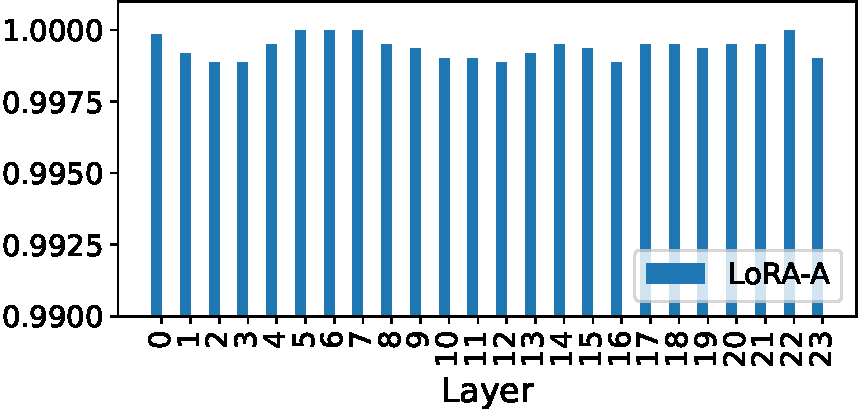
\includegraphics[width=0.32\linewidth]{rte_mean_value_iid_lora_A.pdf}}
    \subfigure[moderate non-IID]{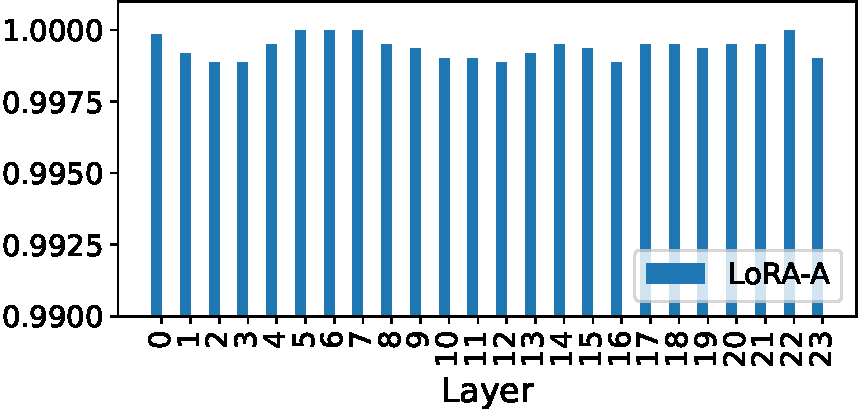
\includegraphics[width=0.32\linewidth]{rte_mean_value_lda_1_lora_A.pdf}}
    \subfigure[server non-IID]{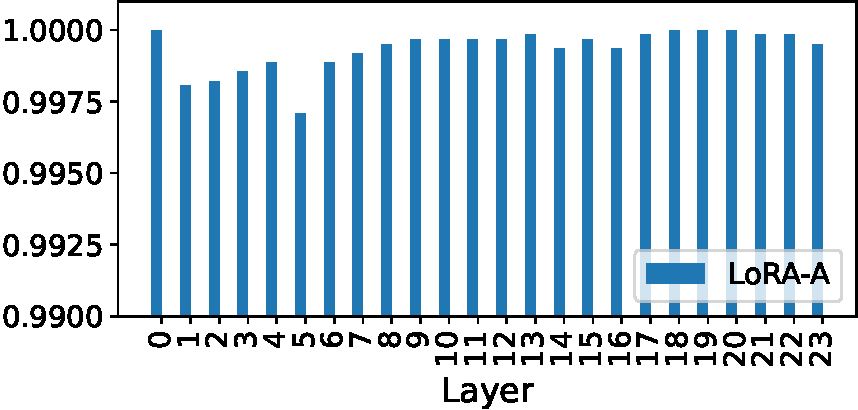
\includegraphics[width=0.32\linewidth]{rte_mean_value_lda_0.5_lora_A.pdf}}
    \subfigure[IID]{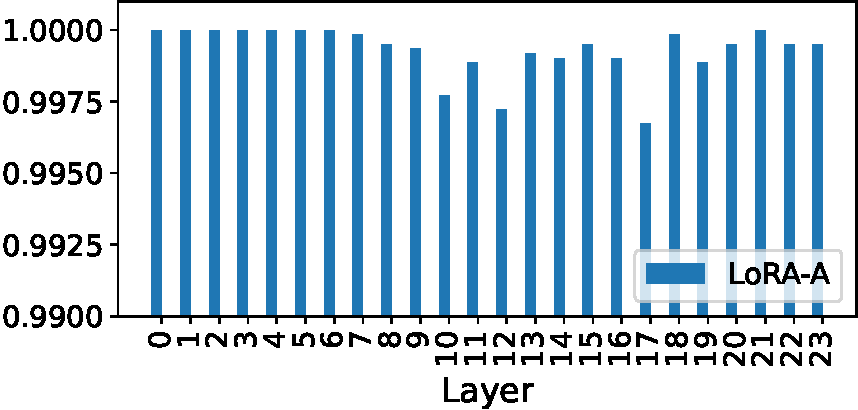
\includegraphics[width=0.32\linewidth]{rte_mean_query_iid_lora_A.pdf}}
    \subfigure[moderate non-IID]{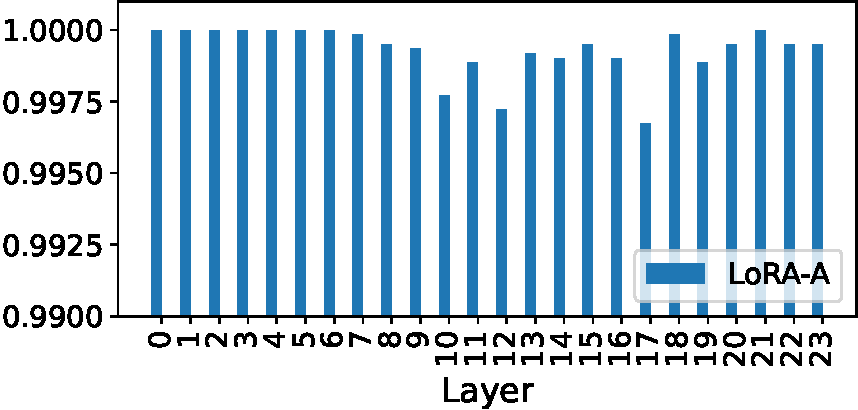
\includegraphics[width=0.32\linewidth]{rte_mean_query_lda_1_lora_A.pdf}}
    \subfigure[server non-IID]{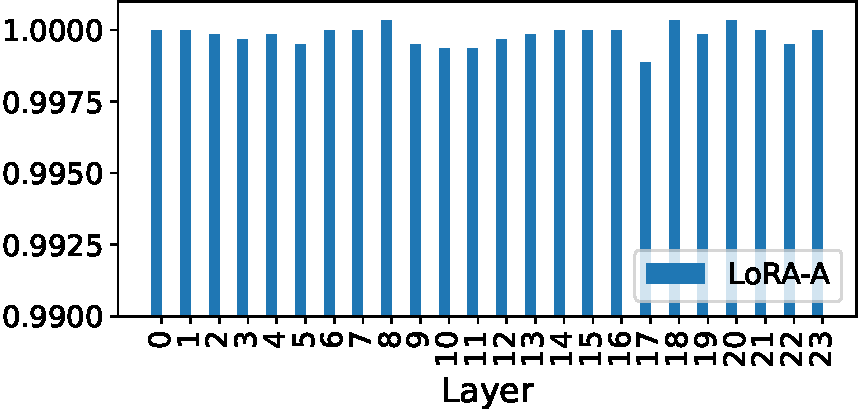
\includegraphics[width=0.32\linewidth]{rte_mean_query_lda_0.5_lora_A.pdf}}
  \caption{Mean of pairwise cosine similarity of the learned $A$ matrices across layers of a RoBERTa model locally fine-tuned with LoRA on the RTE task, with different levels of data heterogeneity. (a)-(c): value matrices; (d)-(f): query matrices. The learned $A$ matrices across client are similar but not identical.}
% \label{fig:motivating_example_value_mean}
\label{fig:motivating_example_mean_A}
\end{figure*}


\begin{figure*}[h]
  \centering
    \subfigure[Client 1 \& Init]{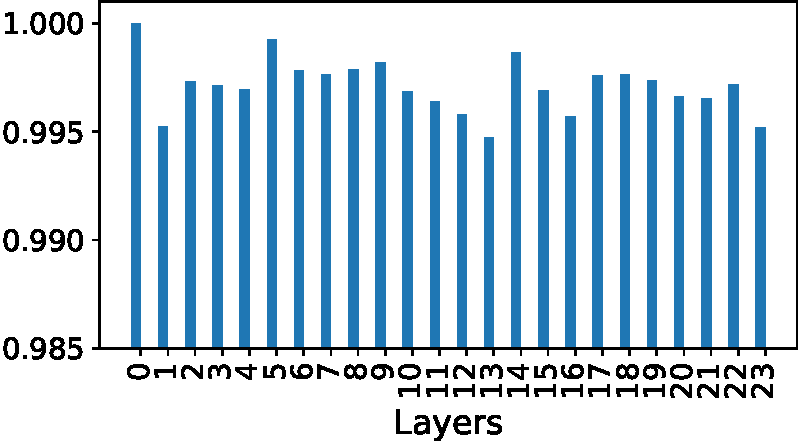
\includegraphics[width=0.32\linewidth]{rte_c1_init_value.pdf}}
    \subfigure[Client 2 \& Init]{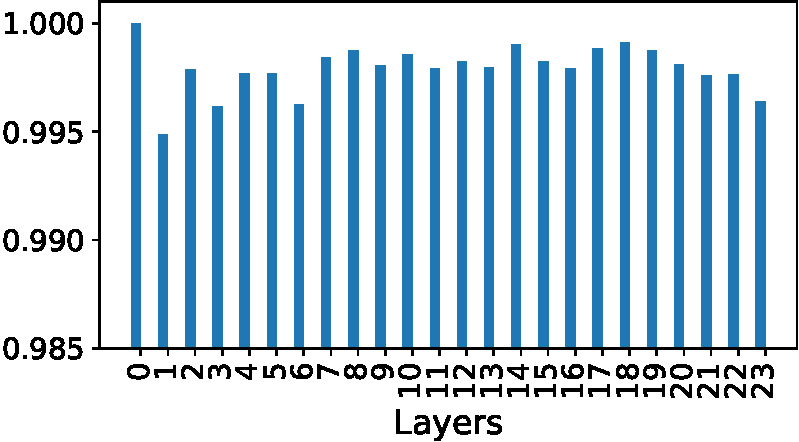
\includegraphics[width=0.32\linewidth]{rte_c2_init_value.pdf}}
    \subfigure[Client 3 \& Init]{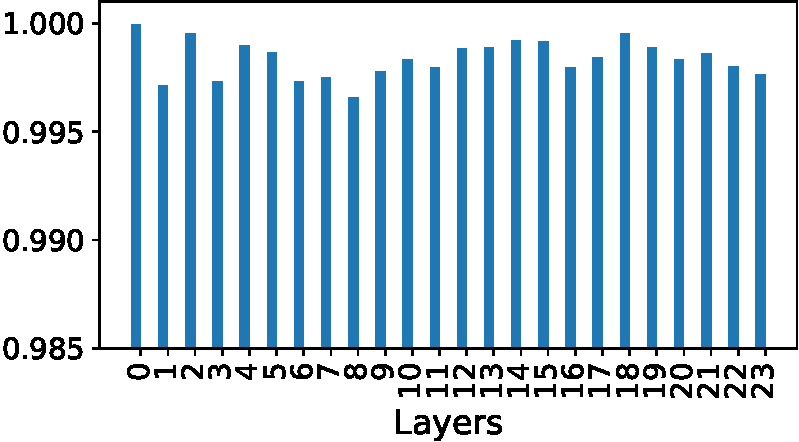
\includegraphics[width=0.32\linewidth]{rte_c3_init_value.pdf}}
    \subfigure[Client 1 \& Init]{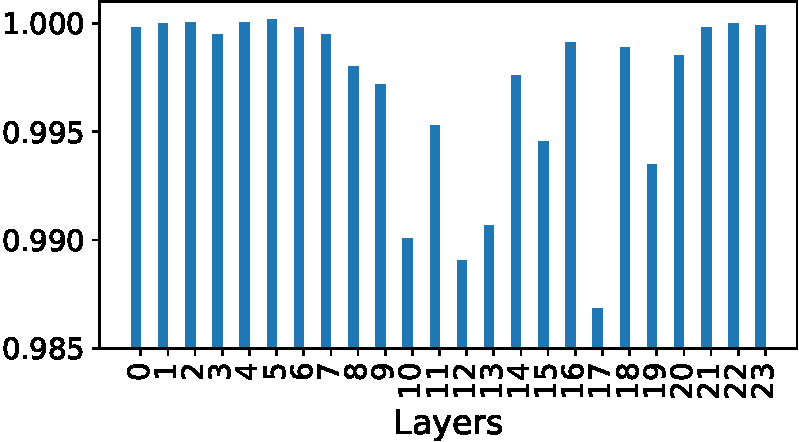
\includegraphics[width=0.32\linewidth]{rte_c1_init_query.pdf}}
    \subfigure[Client 2 \& Init]{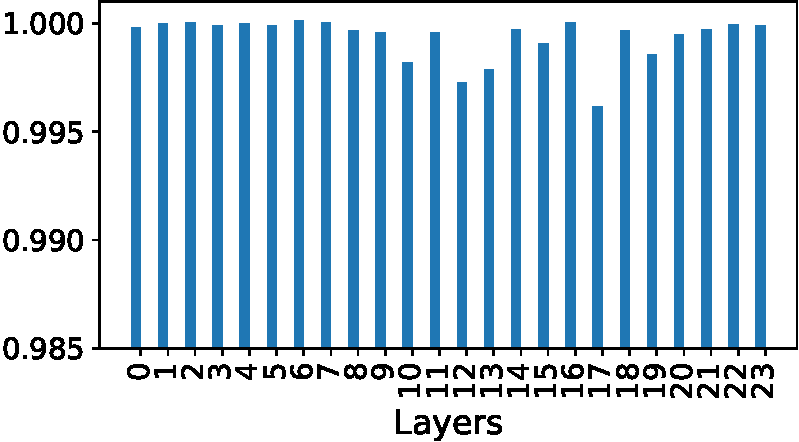
\includegraphics[width=0.32\linewidth]{rte_c2_init_query.pdf}}
    \subfigure[Client 3 \& Init]{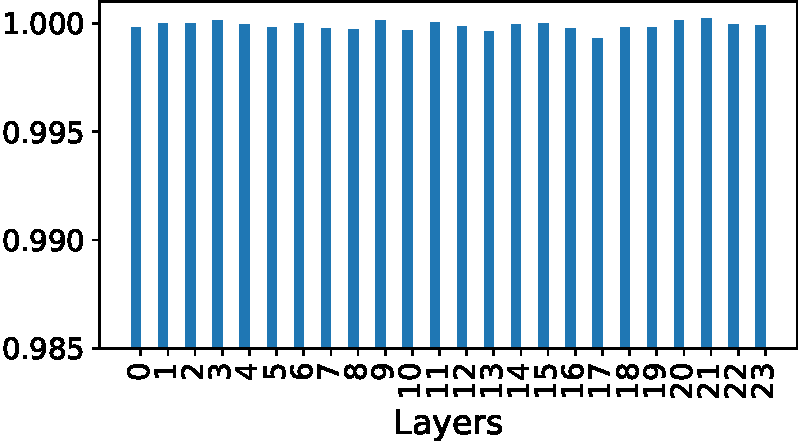
\includegraphics[width=0.32\linewidth]{rte_c3_init_query.pdf}}
  \caption{Cosine similarity of learned and initialized $A$ matrices across layers of different clients of a RoBERTa model locally fine-tuned with LoRA on the RTE task. (a)-(c): value matrices; (d)-(f): query matrices. The learned $A$ matrices are different from the initialized $A$ matrices, indicating that the $A$ matrices are updated.}
\label{fig:motivating_example_init}
\end{figure*}


\subsubsection{Learned rsLoRA Matrices Comparison}

In this section, we present the mean of pairwise client relationships for the learned rsLoRA \citep{kalajdzievski2023rank} matrices. These results, shown in Figure \ref{fig:motivating_example_mean_rslora}, demonstrate a similar phenomenon to the learned LoRA matrices. That is, the learned $A$ matrices are more similar across clients than the $B$ matrices, and with increased data heterogeneity, the similarity of $B$ matrices between different clients decreases.

\begin{figure*}[h]
  \centering
    \subfigure[IID]{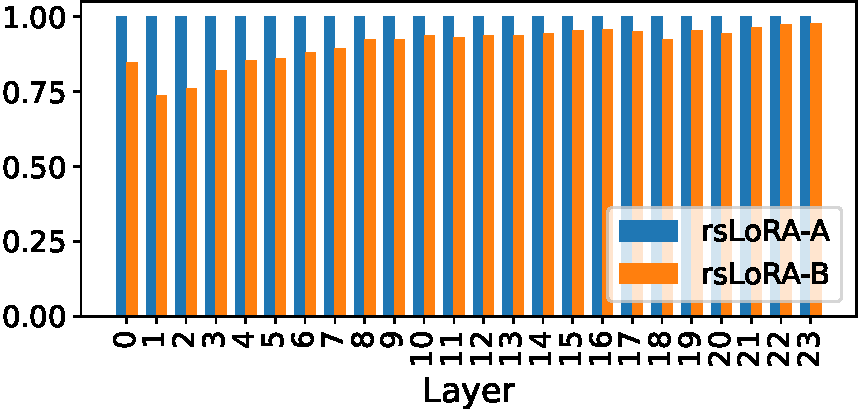
\includegraphics[width=0.32\linewidth]{rte_mean_value_iid_rslora.pdf}}
    \subfigure[moderate non-IID]{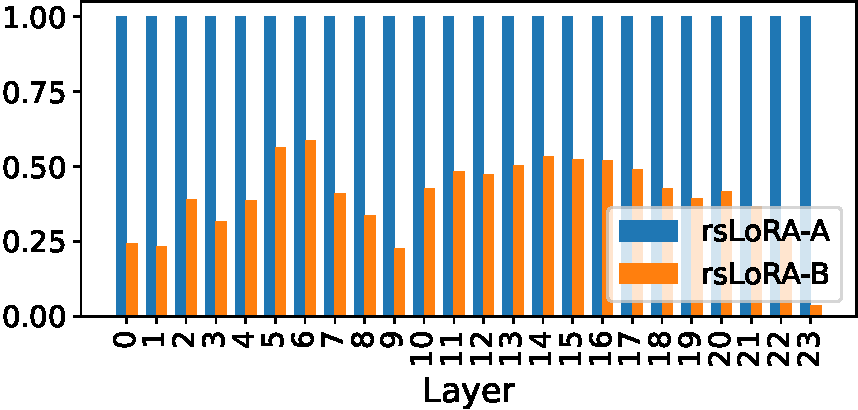
\includegraphics[width=0.32\linewidth]{rte_mean_value_lda_1_rslora.pdf}}
    \subfigure[server non-IID]{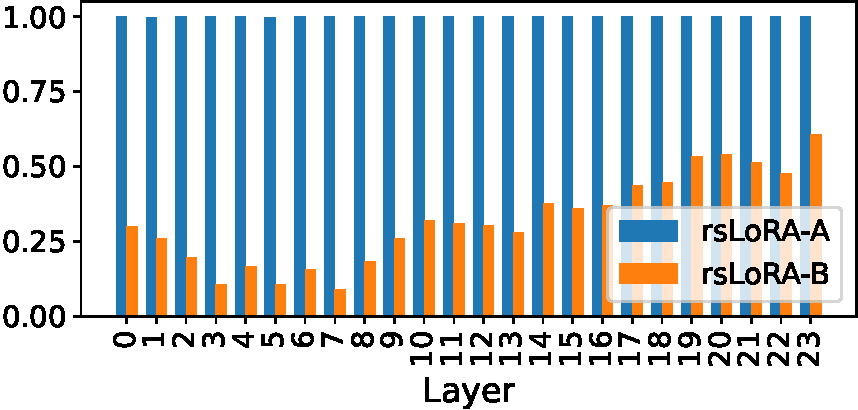
\includegraphics[width=0.32\linewidth]{rte_mean_value_lda_0.5_rslora.pdf}}
    \subfigure[IID]{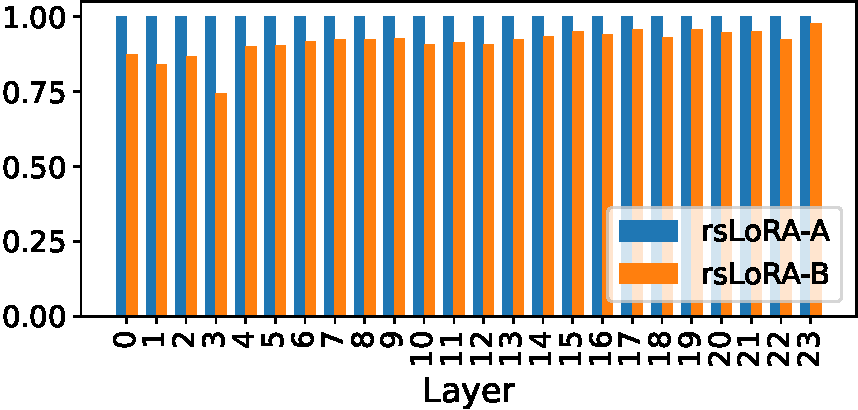
\includegraphics[width=0.32\linewidth]{rte_mean_query_iid_rslora.pdf}}
    \subfigure[moderate non-IID]{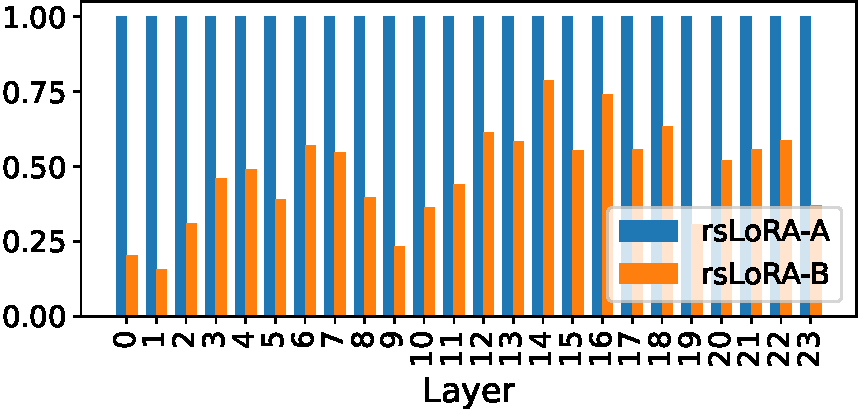
\includegraphics[width=0.32\linewidth]{rte_mean_query_lda_1_rslora.pdf}}
    \subfigure[server non-IID]{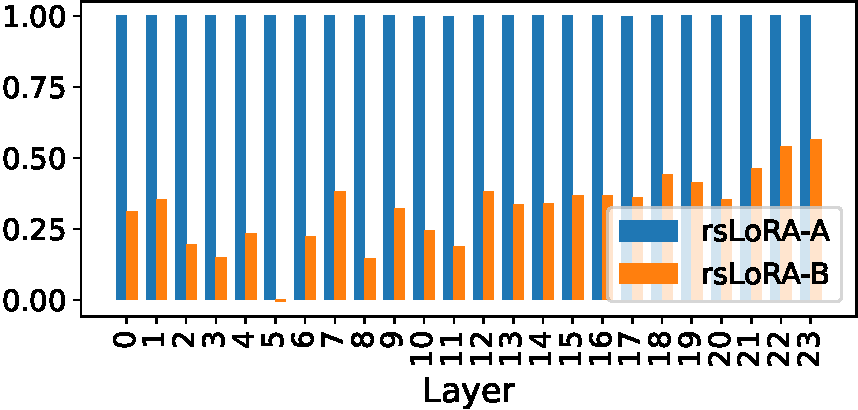
\includegraphics[width=0.32\linewidth]{rte_mean_query_lda_0.5_rslora.pdf}}
  \caption{Mean of pairwise cosine similarity of the learned $A$ and $B$ matrices across layers of a RoBERTa model locally fine-tuned with rsLoRA on the RTE task, with different levels of data heterogeneity. (a)-(c): value matrices; (d)-(f): query matrices. The learned $A$ matrices are more similar across clients than the $B$ matrices, and with increased data heterogeneity, the similarity of $B$ matrices between different clients decreases.}
\label{fig:motivating_example_mean_rslora}
\end{figure*}


\subsubsection{Learned VeRA Matrices Comparison}


In this section, we show the mean of pairwise client relationships for the learned VeRA \citep{kopiczko2024vera} matrices. In VeRA, the low-rank matrices $A$ and $B$ are initialized using the uniform version of Kaiming initialization, fixed, shared across all layers, and adapted with trainable scaling vectors $d$ and $b$. The $b$ vectors are initialized to zero, and the $d$ vectors are initialized with a value of 0.1. To make the notation consistent with our work, we rewrite the scaling vectors $d$ and $b$ as $A_d$ and $B_b$ to reflect the position of each scaling vector. These results, illustrated in Figure \ref{fig:motivating_example_mean_vera}, demonstrate a similar phenomenon to the learned LoRA matrices. That is, the learned scaling vectors $A_d$ are more similar across clients than the scaling vectors $B_b$, and with increased data heterogeneity, the similarity of scaling vectors $B_b$ between different clients decreases.


\begin{figure*}[h]
  \centering
    \subfigure[IID]{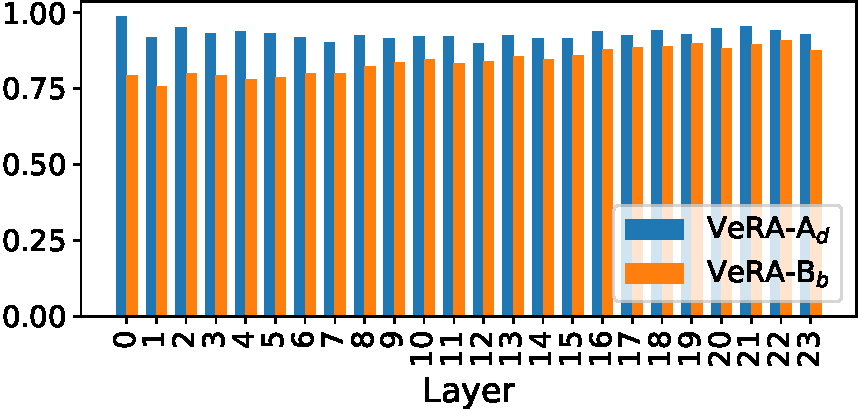
\includegraphics[width=0.32\linewidth]{rte_mean_value_iid_vera.pdf}}
    \subfigure[moderate non-IID]{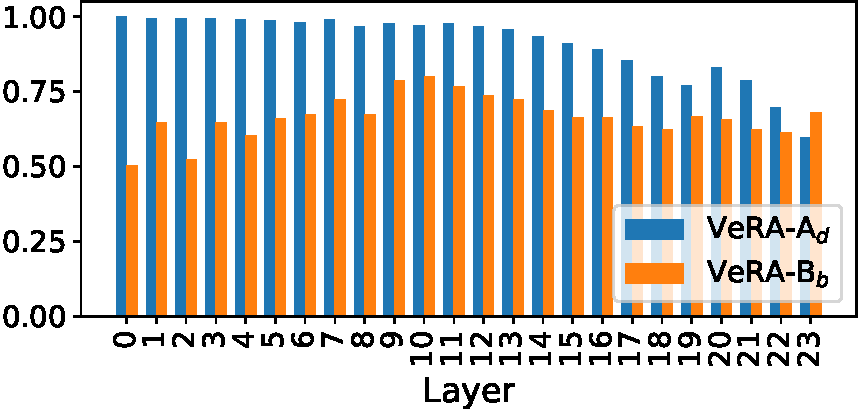
\includegraphics[width=0.32\linewidth]{rte_mean_value_lda_1_vera.pdf}}
    \subfigure[server non-IID]{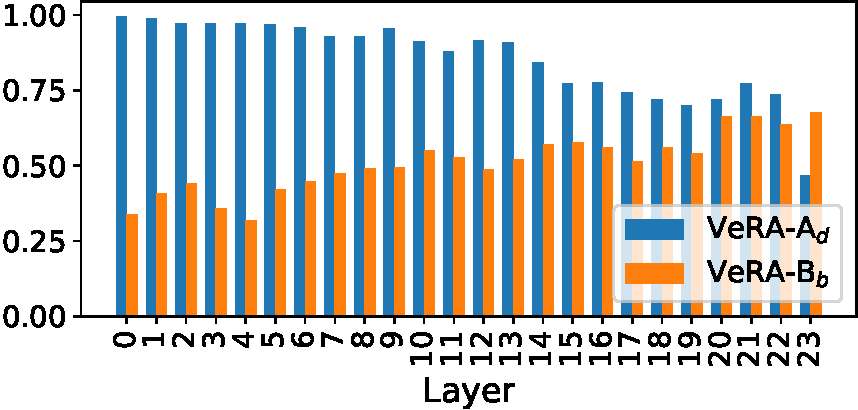
\includegraphics[width=0.32\linewidth]{rte_mean_value_lda_0.5_vera.pdf}}
    \subfigure[IID]{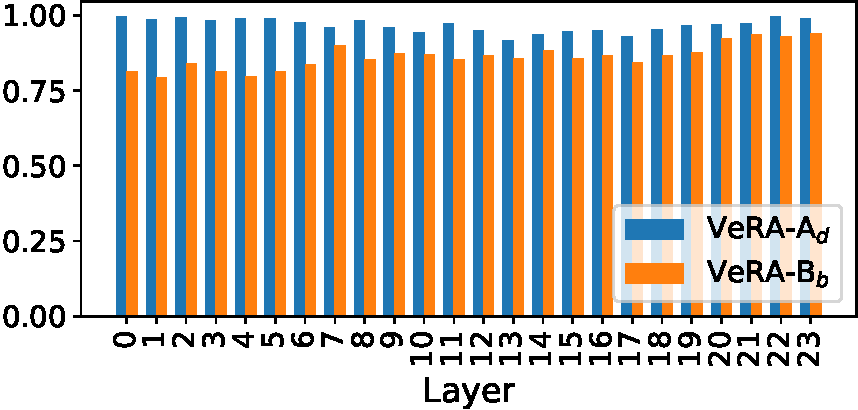
\includegraphics[width=0.32\linewidth]{rte_mean_query_iid_vera.pdf}}
    \subfigure[moderate non-IID]{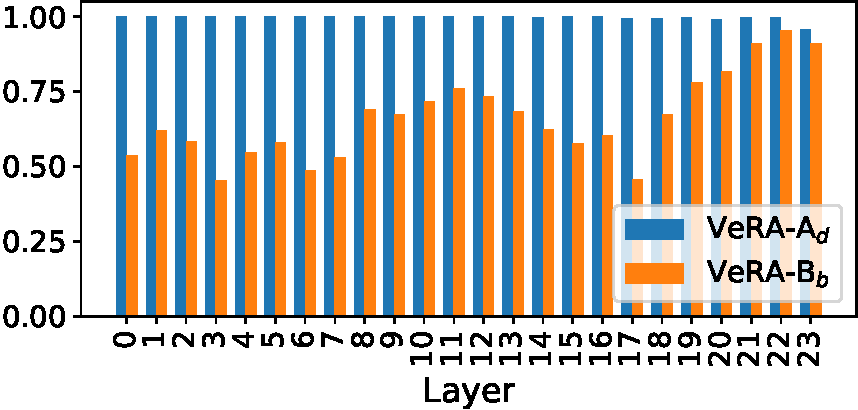
\includegraphics[width=0.32\linewidth]{rte_mean_query_lda_1_vera.pdf}}
    \subfigure[server non-IID]{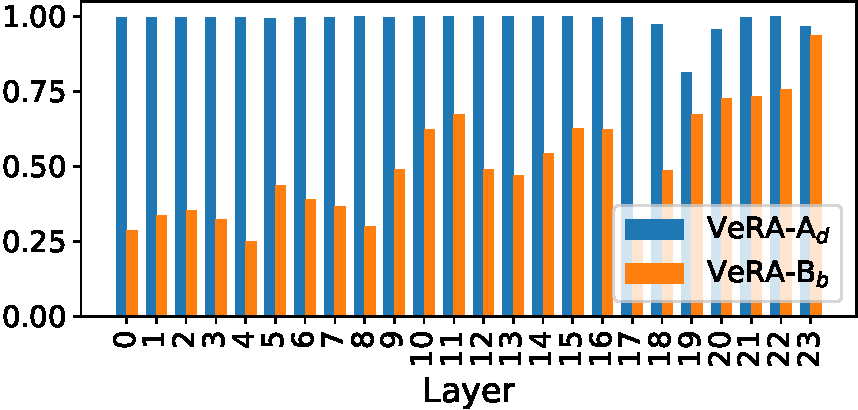
\includegraphics[width=0.32\linewidth]{rte_mean_query_lda_0.5_vera.pdf}}
  \caption{Mean of pairwise cosine similarity of the learned scaling vectors $A_d$ and $B_b$ across layers of a RoBERTa model locally fine-tuned with VeRA on the RTE task, with different levels of data heterogeneity. (a)-(c): value matrices; (d)-(f): query matrices. The learned scaling vectors $A_d$ are more similar across clients than the scaling vectors $B_b$, and with increased data heterogeneity, the similarity of scaling vectors $B_b$ between different clients decreases.}
\label{fig:motivating_example_mean_vera}
\end{figure*}


\subsection{Further Results on Compressing $A$ matrices}

Based on the reviewers' comments during the review stage, we further conduct experiments on compressing the $A$ matrices. Specifically, we chose FetchSGD \citep{rothchild2020fetchsgd} to compress around 50\% of the $A$ matrices, given that the updates across the $A$ matrices are trivial but necessary. The experimental results are shown in Table \ref{tab:compress}, which indicates that FedSA-LoRA with a compression method achieves performance comparable to the original FedSA-LoRA. This confirms that the $A$ matrices can indeed be further compressed to reduce communication overhead while maintaining satisfactory performance, validating the reviewer’s hypothesis that ``there must exist a compression method or a sparse structure to significantly reduce the number of parameters in the $A$ matrices that need to be updated''. 


\begin{table}[h]
\caption{Time and space costs for each method on the RTE and QNLI tasks. \# Communication round denotes the number of communication rounds to reach the predefined target performance. $^{\ddagger}$ denotes equipped with the compressing method FetchSGD.}
\label{tab:compress}
\begin{center}
\resizebox{\linewidth}{!}{
\begin{tabular}{lcccccccc}
\toprule 
& \multirow{2}{*}{\# Trainable Parm.} &  \multirow{2}{*}{\# Per-round Communicated Parm.}  & \multicolumn{2}{c}{\# Per-round Computation Cost} & \multicolumn{2}{c}{\# Communication Round} & \multicolumn{2}{c}{Accuracy} \\
 \cmidrule(lr){4-5}  \cmidrule(lr){6-7}  \cmidrule(lr){8-9}
& & & RTE & QNLI & RTE & QNLI  & RTE & QNLI \\
\midrule
LoRA & 1.83M & 0.78M & 22s & 35s & 167 & 397 & $87.49_{\pm 0.15}$ & $91.16_{\pm 0.72}$ \\
FFA-LoRA & 1.44M & 0.39M & 20s & 33s & 229 & 374  & $86.08_{\pm 1.16}$ & $91.52_{\pm 0.59}$ \\
FedDPA-LoRA & 2.62M & 0.78M & 23s & 37s &  128 & 325  & $87.44_{\pm 0.13}$ & $90.74_{\pm 1.38}$ \\
\midrule
FedSA-LoRA & 1.83M & 0.39M & 22s & 34s &  91 & 224  & $87.93_{\pm 0.11}$ & $92.13_{\pm 0.24}$ \\
FedSA-LoRA$^{\ddagger}$ & 1.83M & 0.20M & 22s	& 34s & 79 & 155  & $87.88_{\pm 0.13}$ & $92.16_{\pm 0.20}$  \\
\bottomrule
\end{tabular}
}
\end{center}
\end{table}
